\documentclass[proposal,indonesia]{ugmskripsi}
% Options:
%   skripsi / proposal        (default: skripsi)
%   satuspasi / duaspasi / satusetengahspasi (default: satusetengahspasi)
%   indonesia / inggris       (default: indonesia)

%------------------------------------------------------------
% Metadata Proposal
%------------------------------------------------------------
% TODO: Ganti metadata di bawah ini dengan data Anda sendiri
\titleind{ANALISIS ATENSI VISUAL PADA ANTARMUKA OPENIMIS MENGGUNAKAN MODEL SALIENCY PREDICTION}
\titleeng{VISUAL ATTENTION ANALYSIS ON OPENIMIS INTERFACE USING SALIENCY PREDICTION MODEL}
\fullname{KHAIRUMAYZAL DWIKSANENDRA}
\idnum{23/513946/PA/21969}
\degree{JENJANG}
\gelar{GELAR}
\yearsubmit{2026}
\program{ILMU KOMPUTER}
\dept{DEPARTEMEN ILMU KOMPUTER DAN ELEKTRONIKA}
\firstsupervisor{NAMA DOSEN PEMBIMBING}
\firstexaminer{NAMA DOSEN PENGUJI 1}
\secondexaminer{NAMA DOSEN PENGUJI 2}

%------------------------------------------------------------
% Packages
%------------------------------------------------------------
\usepackage[utf8]{inputenc}
\usepackage{graphicx}
\graphicspath{{figures/}}
\usepackage{amsmath}
\usepackage{amssymb}
\usepackage{booktabs}
\usepackage{longtable}
\usepackage{tabularx}
\usepackage{multirow}
\usepackage{float}
\usepackage{listings}
\usepackage{xcolor}
\usepackage{hyperref}
\usepackage{url}
\usepackage{enumitem}

% Code listing style
\lstset{
    basicstyle=\ttfamily\small,
    breaklines=true,
    frame=single,
    numbers=left,
    numberstyle=\tiny,
    keywordstyle=\color{blue},
    commentstyle=\color{gray},
    stringstyle=\color{orange},
    showstringspaces=false,
    tabsize=2
}

% Define YAML language for listings
\lstdefinelanguage{yaml}{
  keywords={true,false,null,y,n},
  sensitive=false,
  comment=[l]{\#},
  morecomment=[s]{/*}{*/},
  morestring=[b]',
  morestring=[b]"
}

% Define Docker language for listings
\lstdefinelanguage{docker}{
  alsoletter={-},
  keywords={FROM,RUN,CMD,LABEL,MAINTAINER,EXPOSE,ENV,ADD,COPY,ENTRYPOINT,VOLUME,USER,WORKDIR,ARG,ONBUILD,STOPSIGNAL,HEALTHCHECK,SHELL},
  sensitive=false,
  comment=[l]{\#},
  morestring=[b]',
  morestring=[b]"
}

%------------------------------------------------------------
% Document Body
%------------------------------------------------------------
\begin{document}

% Preliminary Pages (Proposal: minimal)
\cover
\titlepageind
\approvalpage

\tableofcontents

\abstractind
% TODO: Tulis intisari dalam Bahasa Indonesia di sini (150-250 kata).
% Jelaskan latar belakang, tujuan, metode, dan hasil penelitian.

Antarmuka sistem administrasi kesehatan berbasis web seperti openIMIS berisi elemen informasi yang kritis secara operasional dan finansial, seperti status kelayakan peserta, indikator potensi penipuan, dan status klaim, namun tidak ada jaminan bahwa elemen-elemen tersebut secara alami menarik atensi visual pengguna saat berinteraksi dengan antarmuka. Riset di bidang human-computer interaction menunjukkan bahwa hambatan adopsi sistem informasi kesehatan tidak semata soal infrastruktur, melainkan juga usability antarmuka \citep{verma2021openmrs,paton2022open}. Meskipun model deep learning untuk prediksi atensi visual (saliency) pada antarmuka digital telah berkembang matang lebih dari satu dekade, penerapannya secara spesifik pada antarmuka sistem administrasi kesehatan seperti openIMIS belum ditemukan pada literatur yang tersedia. Penelitian ini bertujuan mengembangkan sebuah alat diagnostik berbasis model prediksi atensi visual pra-latih, tanpa fine-tuning menggunakan data domain, untuk mengevaluasi kesesuaian antara zona atensi visual prediktif dengan lokasi elemen kritis pada antarmuka openIMIS. Akurasi umum model diuji lebih dahulu pada benchmark publik UEyes, khususnya kategori Webpage dan Desktop UI, sebagai ukuran kredibilitas umum. Model kemudian diterapkan pada tangkapan layar openIMIS untuk menghasilkan peta atensi, yang dibandingkan dengan elemen kritis hasil pelabelan pakar domain, lalu divalidasi lebih lanjut melalui sesi tinjauan kualitatif bersama pakar. Alat yang dihasilkan berupa aplikasi web sederhana yang menerima unggahan tangkapan layar dan menghasilkan visualisasi peta atensi secara otomatis. Penelitian ini diharapkan memberikan kontribusi metodologis awal dalam mendiagnosis risiko desain antarmuka sistem administrasi kesehatan tanpa memerlukan data eye-tracking domain-spesifik yang mahal untuk dikumpulkan.
\\

\noindent \textbf{Kata Kunci:} 
\newline 
Visual Attention Prediction, Saliency, Human-Computer Interaction, openIMIS, Deep Learning, Zero-Shot Learning, Health Information Systems, UEyes
\endabstractind

\abstracteng
% TODO: Write abstract in English here (150-250 words).
% Explain background, objectives, methods, and results.

Lorem ipsum dolor sit amet, consectetur adipiscing elit. Sed do eiusmod tempor incididunt ut labore et dolore magna aliqua. Ut enim ad minim veniam, quis nostrud exercitation ullamco laboris nisi ut aliquip ex ea commodo consequat. Duis aute irure dolor in reprehenderit in voluptate velit esse cillum dolore eu fugiat nulla pariatur.
\endabstracteng

%------------------------------------------------------------
% Chapters
%------------------------------------------------------------
\chapter{PENDAHULUAN}

\section{Latar Belakang}

% TODO: Tulis latar belakang penelitian Anda di sini.
% Jelaskan konteks, urgensi, dan relevansi topik yang dipilih.
% Rujuk pada penelitian terdahulu dan data sekunder jika ada.

Sistem informasi manajemen asuransi kesehatan sumber terbuka seperti openIMIS (\textit{open Insurance Management Information System}) dirancang untuk mendukung proses administratif penjaminan kesehatan, misalnya pendaftaran peserta, penelusuran informasi peserta, dan pengelolaan klaim. openIMIS merupakan perangkat lunak yang telah disertifikasi sebagai digital public good dan dilaporkan digunakan di 14 negara untuk mengelola program yang menjangkau lebih dari 39 juta penerima manfaat, mencakup asuransi kesehatan, asuransi kecelakaan kerja, transfer tunai, dan skema voucer \citet{openimis2026}. Antarmuka sistem semacam ini memuat elemen informasi utama yang menopang pelaksanaan proses tersebut, seperti informasi eligibilitas peserta dan status klaim. Apabila elemen-elemen tersebut tidak berada pada posisi yang secara alami menarik atensi visual pengguna, pelaksanaan proses administratif berpotensi kurang efisien atau kurang tepat, namun sejauh ini belum ada mekanisme sistematis untuk memeriksa apakah elemen informasi utama memang berada pada zona yang diprediksi menarik atensi visual.

Isu ketidaksesuaian antara desain antarmuka dan kebutuhan pengguna dalam sistem informasi kesehatan bukan hal baru. Kajian terhadap implementasi OpenMRS selama 15 tahun di negara berpendapatan rendah dan menengah menemukan bahwa hambatan adopsi sistem rekam medis elektronik tidak hanya perihal infrastruktur, melainkan juga \textit{usability} antarmuka dan rendahnya literasi teknologi informasi tenaga kesehatan, sehingga memerlukan pendekatan \textit{Human-Centered Design} \citep{verma2021openmrs}. Selain itu, kajian pada IMIA Yearbook menegaskan bahwa \textit{resilience, accessibility,} dan \textit{equity} menjadi tiga pilar utama sistem kesehatan digital, dan menyoroti upaya pembangunan ulang arsitektur antarmuka OpenMRS generasi baru dengan pengujian pengguna yang mencakup lintas negara \citep{paton2022open}. Kedua kajian ini menunjukkan bahwa evaluasi \textit{usability} pada sistem informasi kesehatan penting, namun keduanya masih bertumpu pada metode evaluasi konvensional (studi lapangan, pengujian pengguna langsung) yang memerlukan sumber daya besar sehingga sulit direplikasi dalam skala kecil seperti dalam konteks penelitian tugas akhir.

Di sisi lain, bidang prediksi atensi visual (\textit{visual attention/gaze saliency prediction}) berbasis \textit{deep learning} telah berkembang matang selama kurang lebih satu dekade, dengan sejumlah model seperti DeepGaze, UMSI, dan TranSalNet, serta didukung oleh dataset benchmark antarmuka digital berskala besar seperti UEyes yang dipublikasikan pada ACM CHI 2023. Model-model ini memungkinkan estimasi peta atensi visual pada sebuah antarmuka tanpa memerlukan partisipan manusia di setiap sesi pengujian, berbeda dengan pendekatan berbasis riil (misalnya \textit{heatmap} berbasis klik/\textit{mouse-tracking}) yang selama ini lebih umum digunakan dalam evaluasi usabilitas. Karakteristik inilah yang menjadikan model prediksi atensi visual berpotensi sebagai pendekatan analisis yang lebih efisien dari sisi biaya dan waktu dibandingkan studi eye-tracking konvensional.

Meskipun demikian, penelusuran literatur pada Scopus dan IEEE Xplore, penelusuran sitasi lanjut terhadap UEyes pada Scopus dan Google Scholar, serta pencarian web eksploratori pada Oktober 2026 (selanjutnya disebut literatur yang ditelusuri) belum menemukan studi yang menerapkan model prediksi atensi visual pada antarmuka sistem informasi kesehatan administratif, termasuk pada openIMIS. Studi pada domain kesehatan dan asuransi yang ditemukan umumnya memakai pelacakan mata secara manual atau menganalisis citra diagnostik.Kekosongan ini konsisten dengan kendala praktis di lapangan: tidak tersedia dataset eye-tracking atau data interaksi pengguna openIMIS yang dapat dijadikan basis pelatihan atau validasi kuantitatif standar (metrik seperti NSS, CC, atau KLD), dan pengumpulan data semacam itu secara mandiri berada di luar kelayakan waktu dan sumber daya penelitian tugas akhir tingkat sarjana. Akses ke pengguna operasional maupun pakar domain untuk keperluan validasi juga sulit diperoleh.

Untuk menjawab kendala tersebut, penelitian ini mengusulkan pendekatan yang tidak bergantung pada \textit{fine-tuning} berbasis data domain-spesifik. Model prediksi atensi visual pra-latih (\textit{pretrained}), yaitu TranSalNet\_Res, digunakan langsung tanpa modifikasi bobot. Kredibilitas umum model diuji terlebih dahulu pada benchmark publik UEyes, khususnya kategori \textit{Webpage} dan \textit{Desktop UI} yang secara struktural paling mendekati antarmuka openIMIS, sebagai tolok ukur independen, bukan sebagai basis pelatihan untuk domain openIMIS. Model yang sama kemudian diterapkan pada tangkapan layar openIMIS untuk menghasilkan peta atensi. Skor saliency prediktif pada area setiap elemen antarmuka, yang kotaknya diambil dari struktur halaman (\textit{Document Object Model}/DOM), selanjutnya dibandingkan antara elemen informasi utama, yang dilabeli secara sistematis dari dokumentasi resmi, materi pelatihan, dan video demonstrasi openIMIS menggunakan buku kode yang terdokumentasi, dan elemen yang tidak berlabel. Perlu ditegaskan bahwa model yang digunakan memprediksi atensi visual yang bersifat \textit{bottom-up} pada kondisi pengamatan bebas (\textit{free-viewing}), sebagaimana data acuan UEyes yang dikumpulkan tanpa tugas spesifik (Jiang et al., 2023), sehingga hasil penelitian ini hanya menyatakan tingkat menonjolnya elemen secara visual (saliency) menurut prediksi model dan tidak mengklaim perilaku pengguna yang sedang mengerjakan tugas. Topik penelitian ini memiliki relevansi kuat dengan roadmap riset \textit{Human-Computer Interaction} dan penerapan kecerdasan buatan pada sistem informasi kesehatan di Departemen Ilmu Komputer dan Elektronika FMIPA UGM, khususnya arah riset yang dikembangkan pada Lab Rekayasa Perangkat Lunak dan Data. Riset ini diharapkan dapat memberikan kontribusi metodologis maupun praktis terhadap diagnosis risiko desain antarmuka pada sistem informasi kesehatan administratif.


\section{Rumusan Masalah}

% TODO: Tulis rumusan masalah dalam bentuk pertanyaan penelitian.
% Rumusan masalah harus spesifik, terukur, dan dapat dijawab.

Berdasarkan latar belakang yang telah diuraikan, dapat dirumuskan permasalahan penelitian sebagai berikut:
\begin{enumerate}
  \item Antarmuka sistem administrasi kesehatan seperti openIMIS memuat elemen informasi utama yang menopang pelaksanaan proses administratif, namun tingkat menonjolnya elemen tersebut secara visual dalam peta atensi visual prediktif perlu dievaluasi secara sistematis.
  \item Model \textit{deep learning} untuk prediksi atensi visual telah berkembang matang pada berbagai domain antarmuka digital umum, namun belum ditemukan acuan mengenai penerapannya pada antarmuka sistem administrasi kesehatan berbasis asuransi pada literatur yang ditelusuri, sehingga tingkat kredibilitas model pra-latih TranSalNet\_Res pada benchmark publik UEyes kategori \textit{Webpage} dan \textit{Desktop UI} perlu diukur sebagai dasar menafsirkan peta atensi pada antarmuka openIMIS.
  \item Ketidaktersediaan dataset \textit{eye-tracking} atau data interaksi pengguna yang spesifik pada domain openIMIS menjadi kendala untuk validasi kuantitatif standar (NSS/CC/KLD) untuk model prediksi atensi visual, sehingga diperlukan pendekatan metodologis alternatif yang transparan dan dapat direplikasi untuk membandingkan atensi visual prediktif dengan elemen informasi utama, tanpa memerlukan fine-tuning berbasis data domain dan tanpa validasi pakar.
\end{enumerate}

\section{Batasan Masalah}

% TODO: Tulis batasan masalah untuk memfokuskan penelitian.
% Batasan dapat mencakup ruang lingkup, teknologi, atau aspek yang tidak diteliti.

Untuk menjaga fokus dan kelayakan penelitian dalam lingkup tugas akhir, ditetapkan batasan sebagai berikut:

\begin{enumerate}
  \item Objek studi dibatasi pada antarmuka sistem openIMIS versi \textit{sandbox}/demo, bukan lingkungan produksi aktif
  \item Model prediksi atensi visual yang digunakan adalah TranSalNet\_Res pra-latih \textit{open-source} tanpa \textit{fine-tuning} tambahan menggunakan data domain openIMIS. Model lain (mis. TranSalNet\_Dense, SUM) dan pendekatan zero-shot berbasis model visual-language berada di luar cakupan inti dan hanya disebut sebagai pengembangan lanjutan.
  \item Validasi akurasi umum model dilakukan dengan publik UEyes, khusus kategori \textit{Webpage} dan \textit{Desktop UI}, sebagai ukuran kredibilitas umum dan bukan sebagai metrik akurasi domain spesifik openIMIS
  \item Elemen informasi utama pada antarmuka openIMIS ditentukan melalui pelabelan oleh satu pelabel (peneliti) berdasarkan buku kode yang terdokumentasi, dengan sumber berupa dokumentasi resmi, materi pelatihan, dan video demonstrasi resmi openIMIS. Suatu elemen dilabeli apabila didukung oleh minimal dua sumber. Penelitian ini tidak melibatkan validasi oleh pakar atau pengguna operasional, sehingga hasilnya bersifat eksploratif dan tidak mengklaim kesesuaian dengan perilaku pengguna nyata.
  \item Sumber pelabelan dan tangkapan layar dapat berasal dari versi antarmuka yang berbeda. Pemetaan elemen dilakukan berdasarkan fungsinya, dan perbedaan versi dinyatakan sebagai keterbatasan penelitian.
  \item Luaran penelitian berupa analisis yang dituangkan dalam laporan skripsi; penelitian tidak mencakup pengembangan aplikasi atau perangkat lunak bagi pengguna akhir. Inferensi model, perhitungan skor saliency per elemen, dan analisis statistik dikerjakan melalui skrip analisis (\textit{notebook}) yang didokumentasikan sebagai instrumen penelitian. Pengembangan backend/infrastruktur openIMIS itu sendiri berada di luar cakupan penelitian.
  \item Penelitian tidak mencakup siklus \textit{redesign} penuh terhadap antarmuka openIMIS, keluaran penelitian adalah analisis tingkat menonjolnya elemen secara visual dan kandidat rekomendasi, bukan implementasi ulang desain.
  \item Validasi kuantitat skala kecil dengan partisipan proksi (5-10 orang) merupakan opsi penguat apabila logistik memungkinkan, bukan komponen wajib penelitian.
  \item Cakupan layar dibatasi pada sejumlah alur tugas yang dipilih berdasarkan kriteria kecukupan sumber (dijelaskan pada Bab 3), dan analisis hanya mencakup elemen pada viewport awal setiap layar.
  \item Klaim penelitian dibatasi pada atensi visual prediktif (bottom-up, free-viewing); penelitian tidak mengklaim perilaku atau atensi pengguna yang sedang mengerjakan tugas.
\end{enumerate}

\section{Tujuan Penelitian}

% TODO: Tulis tujuan penelitian yang ingin dicapai.
% Tujuan harus sesuai dengan rumusan masalah.

Berdasarkan rumusan masalah dan batasan yang telah diidentifikasi, tujuan penelitian ini adalah:

\begin{enumerate}
  \item Mengukur kredibilitas umum model prediksi atensi visual yang dipilih melalui benchmark publik UEyes pada kategori \textit{Webpage} dan \textit{Desktop UI}
  \item Membandingkan tingkat menonjolnya secara visual (berdasarkan skor saliency prediktif) elemen informasi utama dengan elemen tidak berlabel pada antarmuka openIMIS, berdasarkan pelabelan dari dokumentasi resmi, materi pelatihan, dan video demonstrasi, menggunakan ukuran persentil dan uji permutasi dengan hipotesis dua arah.
  \item Merumuskan temuan beserta kandidat rekomendasi perbaikan tata letak antarmuka yang memerlukan pengujian lanjutan dengan pengguna, dengan menyatakan keterbatasan validasinya secara eksplisit.
\end{enumerate}


\section{Manfaat Penelitian}

% TODO: Tulis manfaat penelitian bagi akademik dan praktis.

Penelitian ini diharapkan memberikan manfaat sebagai berikut:

\begin{enumerate}
  \item \textbf{Bagi akademik:} memberikan kontribusi metodologis awal pada irisan bidang prediksi atensi visual dan desain antarmuka sistem informasi kesehatan administratif, sebuah gap yang belum ditemukan pada literatur yang ditelusuri.
  \item \textbf{Bagi pengembang/pengelola openIMIS:} menyediakan pendekatan penelusuran awal yang efisien dari sisi biaya dan waktu untuk mengidentifikasi kandidat risiko desain antarmuka yang perlu diuji lebih lanjut dengan pengguna, tanpa memerlukan pengumpulan data eye-tracking yang berbiaya tinggi dan berdurasi panjang, dan bukan sebagai pengganti uji pengguna.
  \item \textbf{Bagi komunitas pengembang dan pengelola sistem informasi asuransi kesehatan \textit{open source}:}Menjadi dasar awal bagi kajian usability lanjutan yang lebih besar dan berbasis data domain-spesifik di pengembangan selanjutnya.
  \item \textbf{Bagi peneliti selanjutnya:} memberikan \textit{baseline} metodologi (validasi \textit{benchmark} umum dan expert judgment tanpa \textit{fine-tuning}) yang berpotensi direplikasi pada domain sistem informasi lain dengan keterbatsan data serupa. 
\end{enumerate}


\chapter{PENELITIAN TERKAIT}

\section{Konsep Atensi Visual dan Prediksi Saliency}

% TODO: Jelaskan teori atau konsep pertama yang relevan dengan penelitian Anda.
% Gunakan referensi dari pustaka yang terpercaya.

Konsep \textit{saliency} dalam konteks atensi visual pertama kali diformalkan secara komputasional oleh \citet{itti1998model} melalui model \textit{bottom-up} yang terinspirasi dari arsitektur neuronal sistem visual primata. Model ini menggabungkan fitur intensitas, orientasi, dan warna dari sebuah citra ke dalam satu peta topografis (\textit{saliency map}) yang merepresentasikan seberapa besar kemungkinan suatu lokasi menarik atensi visual manusia secara alami tanpa dipengaruhi oleh tugas atau tujuan kognitif tertentu \citep{itti1998model}. Model-model generasi awal ini menjadi fondasi konseptual bagi seluruh perkembangan riset prediksi atensi visual selanjutnya, termasuk model berbasis deep learning yang lebih modern dan dibahas pada subbab 2.2.

Istilah \textit{``Saliency''} pada riset ini merujuk secara spesifik pada prediksi atensi visual/gaze, yaitu upaya memodelkan ke mana mata manusia secara alami akan tertarik ketika melihat sebuah antarmuka atau citra. Istilah ini perlu dibedakan dari penggunaan kata \textit{``saliency''} pada bidang riset yang berbeda, yaitu \textit{explainability} atau \textit{Explainable AI} (XAI), dimana teknik seperti \textit{Gradient-weight Class Activation Mapping} (Grad-CAM) digunakan untuk menghasilkan peta yang menyoroti wilayah citra mana yang paling memengaruhi keputusan klasifikasi sebuah model \textit{deep learning}, misalnya menjelaskan bagian citra X-ray mana yang mendorong model mendiagnosis suatu penyakit \citep{selvaraju2017grad}. Kedua bidang ini sama-sama menghasilkan keluaran visual berupa peta panas (heatmap), namun secara fundamental berbeda berdasarkan apa yang sedang dimodelkan. Peta atensi visual memodelkan persepsi dan perhatian mata manusia, sedangkan peta \textit{explainability} memodelkan dasar pengambilan keputusan sebuah model AI. Kerancuan antara dua istilah ini merupakan kekeliruan umum dalam penelusuran literatur di bidang ini, sehingga penelitian ini secara konsisten menggunakan istilah \textit{visual attention prediction} atau \textit{gaze/eye-tracking saliency} untuk menghindari ambiguitas tersebut.

Seiring perkembangan \textit{deep learning}, pendekatan prediksi atensi visual bergeser dari model \textit{bottom-up} berbasis fitur tangan (\textit{hand-crafted features}) seperti \citet{itti1998model} menuju model yang dilatih pada data eye-tracking berskala besar untuk mempelajari pola atensi manusia secara \textit{data-driven}. Model-model inilah yang menjadi fokus pembahasan pada subbab berikutnya.

Atensi visual manusia umumnya dipahami dipengaruhi oleh dua kelompok faktor: (1) faktor \textit{bottom-up} yang bersumber dari karakteristik visual stimulus (mis. kontras, warna, dan orientasi, sebagaimana dimodelkan oleh \citealp{itti1998model}) dan (2) faktor \textit{top-down} yang bersumber dari tujuan, tugas, atau pengetahuan pengamat \citep{itti2001computational}. Model prediksi saliency yang dibahas pada subbab berikutnya dilatih dan dievaluasi pada data atensi yang pada umumnya dikumpulkan tanpa tugas spesifik (\textit{free-viewing}; mis. UEyes, \citealp{jiang2023ueyes}; SALICON, \citealp{jiang2015salicon}), karena pengamatan bebas paling lazim dipakai dalam pemodelan saliency \citep{bylinskii2019what}, sehingga keluarannya terutama merepresentasikan komponen yang dapat dipelajari dari tampilan visual semata. Konsekuensinya, pada antarmuka yang digunakan untuk menyelesaikan tugas tertentu seperti openIMIS, peta atensi prediktif tidak dapat disamakan dengan pola atensi pengguna yang sedang bertugas. Studi \textit{eye-tracking} pada laman web melaporkan bahwa karakteristik atensi visual bergantung pada tugas yang dikerjakan pengguna \citet{buscher2009what}, sehingga perbedaan antara pengamatan bebas dan pengamatan berbasis tugas perlu diperhitungkan dalam menafsirkan hasil.


\section{Model Prediksi Saliency Berbasis Deep Learning}

Sejak tahun 2014, \textit{transfer learning} dari jaringan yang telah dilatih pada \textit{classification task} citra berskala besar (mis. ImageNet) menjadi pendorong utama peningkatan akurasi model prediksi saliency, menggantikan pendekatan \textit{bottom-up} berbasis fitur tangan yang dibahas pada subbab sebelumnya. Empat model berikut dipilih sebagai representasi \textit{state of the art} yang relevan bagi penelitian ini, karena seluruhnya tersedia sebagai model \textit{pretrained} yang dapat digunakan langsung tanpa pelatihan ulang. 
 
\begin{enumerate}
    \item \textbf{DeepGaze IIE} \citep{linardos2021deepgaze} dibangun di atas arsitektur DeepGaze II dengan mengganti \textit{backbone} VGG-19 menjadi kombinasi ensemble dari beberapa \textit{backbone} ImageNet yang lebih modern (mis. ResNet-50), digabungkan melalui jaringan \textit{readout} non-linear. Model ini dilatih awal (\textit{pretraining}) pada dataset SALICON (10.000 citra) kemudian di-\textit{fine-tune} pada dataset MIT1003 (citra natural). Karakteristik yang membedakan DeepGaze IIE dari pendahulunya adalah fokus eksplisit pada kalibrasi prediksi, baik pada domain data latih maupun pada domain yang belum pernah dilihat sebelumnya (\textit{out-of-domain}), sebuah properti yang secara langsung relevan dengan konteks penelitian ini, dimana model akan diterapkan pada domain openIMIS yang sama sekali tidak pernah menjadi bagian dari data latihnya.

    \item \textbf{TranSalNet} \citep{lou2022transalnet} mengintegrasikan \textit{encoder} CNN (tersedia dalam dua varian: ResNet-50 pada \textit{TranSalNet\_Res}, atau DenseNet-161 pada \textit{TranSalNet\_Dense}) dengan encoder Transformer yang menerapkan mekanisme \textit{multi-head-self-attention}, digabungkan melalui decoder CNN untuk merekonstruksi peta saliency akhir. Penggabungan ini dirancang agar model dapat menangkap fitur visual lokal (lewat CNN) sekaligus dependensi spasial jarak jauh antar elemen pada citra (lewat Transformer), karakteristik ini berpotensi relevan untuk antarmuka administratif seperti openIMIS yang padat elemen dan tabel data. Model ini dilatih pada dataset SALICON. TranSalNet\_Res dipilih sebagai model utama penelitian karena risiko kebutuhan VRAM yang lebih rendah dibanding TranSalNet\_Dense, dengan performa yang tetap kompetitif menurut evaluasi pada paper aslinya.

    \item \textbf{UMSI (Unified Model of Saliency and Importance)} \citep{fosco2020predicting} secara konseptual sedikit berbeda dari dua model sebelumnya yang memprediksi saliency berbasis fiksasi mata, UMSI memprediksi \textit{visual importance}, dilatih pada dataset Imp1k yang memuat 1.000 desain grafis (mencakup laman web, poster film, antarmuka perangkat mobile, infografis, dan iklan) dengan keterangan kepentingan visual yang dikumpulkan secara \textit{crowdsourced} melalui antarmuka anotasi manual, bukan data \textit{eye-tracking} fisik. UMSI juga dilengkapi modul klasifikasi otomatis untuk mengenali jenis desain input sebelum melakukan prediksi. Model ini penting disebut karena temuan dari \citet{jiang2023ueyes} yang menemukan bahwa ketika UMSI dilatih ulang secara khusus menggunakan data \textit{eye-tracking} UI dari UEyes, akurasinya (AUC) meningkat signifikan dari 0,778 menjadi 0,878, hal ini menjadi sebuah bukti kuantitatif bahwa pelatihan spesifik-domain memberikan pengaruh besar terhadap akurasi prediksi saliency pada antarmuka digital, dan menjadi dasar argumen keterbatasan pada pendekatan \textit{zero-shot} yang diusulkan penelitian ini.
    
    \item \textbf{SUM (Saliency Unification through Mamba)} \citep{hosseini2025sum} adalah model terbaru yang diusulkan, mengintegrasikan arsitektur \textit{Mamba} (\textit{State Space Model}) dengan struktur U-Net serta modul \textit{Conditional Visual State Space} (C-VSS) untuk beradaptasi terhadap berbagai jenis citra dalam satu model tunggal. SUM dilatih secara gabungan pada enam dataset benchmark berskala besar yang mencakup citra natural, laman web, dan citra \textit{e-commerce}. Berdasarkan Tabel 1 pada paper aslinya, salah satu dari enam dataset pelatihan SUM adalah UEyes (dicantumkan sebagai \textit{``U-EYE''}, kategori \textit{Web page}, 1.979 citra dengan 1.583 di antaranya digunakan untuk training), yaitu dataset yang sama yang digunakan sebagai benchmark validasi umum pada pendekatan \textit{zero-shot} tanpa \textit{fine-tuning} yang diusulkan pada Bab 1. Dengan demikian, pengujian SUM pada UEyes tidak dapat dianggap sebagai generalisasi zero-shot yang murni, karena model tersebut telah dilatih menggunakan sebagian data dari dataset yang sama. Temuan ini menjadi pertimbangan tambahan mengapa TranSalNet\_Res, yang tidak dilatih pada UEyes, dipandang sebagai pilihan yang tepat untuk mengukur kredibilitas umum model secara independen pada penelitian ini.
\end{enumerate} 

Secara umum, keempat model yang disebutkan di atas menunjukan pola konsisten di mana seluruhnya mamanfaatkan \textit{transfer learning} dari representasi visual berskala besar (baik dari ImageNet maupun data saliency gabungan), dan tidak dievaluasi atau dilatih khusus pada antarmuka sistem informasi kesehatan administratif seperti openIMIS, sehingga mengonfirmasi kembali kesenjangan yang diidentifikasi pada Bab 1.


\section{Benchmark Saliency pada Antarmuka Digital}

Keempat model yang dibahas pada subbab sebelumnya dievaluasi dan dibandingkan menggunakan dataset benchmark publik. Salah satu dataset yang relevan pagi penelitian ini adalah UEyes \citep{jiang2023ueyes}, sebuah dataset \textit{eye-tracking} berskala besar yang secara khusus dikumpulkan untuk antarmuka digital, bukan citra natural seperti dataset-dataset pendahulunya (SALICON, MIT1003, CAT2000). UEyes terdiri atas 1.980 tangkapan layar antarmuka, dengan masing-masing 495 citra untuk empat kategori UI, yaitu laman web (\textit{webpage}), antarmuka desktop, antarmuka \textit{mobile}, dan poster. Data atensi dikumpulkan dari 62 partisipan menggunakan perangkat \textit{eye-tracker in-lab} beresolusi tinggi (Gazepoint GP3, 60Hz), bukan metode proksi tidak langsung seperti pelacakan kurso mouse atau estimase gaze berbasis webcam yang digunakan pada beberapa dataset saliency sebelumnya. Dataset ini menyediakan peta saliency pada tiga durasi pengamatan (1,3, dan 7 detik) beserta data \textit{scanpath} dan metadata jenis citra untuk tiap sampel.

Evaluasi akurasi model prediksi saliency umumnya dilakukan menggunakan beberapa metrik standar, yang masing-masing mengukur aspek kesesuaian berbeda antara peta saliency hasil prediksi dan data \textit{ground truth}, serta memiliki karakteristik, kelebihan, dan kelemahan yang berbeda satu sama lain \citep{bylinskii2019what}

\begin{enumerate}
    \item \textbf{Correlation Coefficient (CC)} mengukur korelasi linear (Pearson) antara peta prediksi dan peta kepadatan atensi acuan, dengan memperlakukan kedua peta sebagai variabel acak yang dibandingkan secara piksel-demi-piksel. Nilai CC berkisar antara -1 hingga 1, dengan nilai mendekati 1 menunjukan kesesuaian yang semakin baik. Karakteristik penting dari CC adalah sifatnya yang simetris, yaitu memberi bobot penalti yang setara terhadap kesalahan \textit{false positive} (memprediksi atensi tinggi pada area yang sebenarnya tidak diperhatikan) maupun \textit{false negative} (gagal memprediksi atensi tinggi pada area yang sebenarnya diperhatikan)

    \item \textbf{Normalized Scanpath Saliency (NSS)} mengukur nilai rata-rata peta prediksi (setelah dinormalisasi menjadi rata-rata nol dan standar deviasi satu) secara spesifik pada titik-titik lokasi fiksasi aktual pengguna, bukan pada keseluruhan peta. Karena hanya dihitung pada lokasi fiksasi diksrit, NSS lebih sensitif terhadap presisi lokasi dibanding CC. Nilai NSS positif menunjukan kesesuaian prediksi yang lebih baik dari tebakan acak, dan nilai negatif menunjukan prediksi yang justru berlawanan dengan lokasi atensi sebenarnya.

    \item \textbf{Kullback-Leibler Divergence (KLD)} mengukur seberapa besar perbedaan antara dua distribusi probabilitas, yaitu peta prediksi dan peta acuan yang telah dinormalisasi agar jumlah nilainya sama dengan satu. Berbeda dengan CC dan NSS, nilai KLD yang semakin kecil (mendekati nol) menunjukan kesesuaian yang semakin baik. KLD bersifat asimetris sehingga arah perhitungannya menentukan jenis kesalahan yang lebih dihukum. Bila divergensi dihitung dari peta acuan terhadap peta prediksi, sebagaimana konvensi yang dibahas \citet{bylinskii2019what}, penalti lebih besar dijatuhkan pada negatif palsu (area yang diperhatikan pengguna tetapi tidak diprediksi). Implementasi evaluasi resmi UEyes yang diadaptasi pada penelitian ini menghitung divergensi dari peta prediksi terhadap peta acuan, sehingga penalti lebih besar dijatuhkan pada positif palsu (atensi diprediksi pada area yang tidak diperhatikan). Arah yang dipakai dinyatakan eksplisit pada Persamaan (3.7) di Bab 3.

    \item \textbf{Area Under the ROC Curve (AUC)} memperlakukan evaluasi sebagai persoalan klasifikasi biner, yaitu membedakan antara titik fiksasi dan bukan-fiksasi berdasarkan ambang nilai (\textit{treshold}) pada peta prediksi. Nilai AUC berkisat antara 0,5 (setara tebakan acak) hingga 1 (klasifikasi sempurna). Karena berbasis pada peringkat (\textit{ranking}) nilai piksel dan bukan nilai absolutnya, AUC relatif tidak sensitif terhadap skala atau normalisasi peta prediksi, namun beberapa variannya (mis. \textit{shuffled AUC}) perlu digunakan secara hati-hati untuk mengoreksi bias sentral (\textit{center bias}) pada data fiksasi manusia.
\end{enumerate}


Karena masing-masing metrik menangkap aspek kesesuaian yang berbeda, baik dari sisi simetrik/asimetris penalti kesalahan maupun representasi \textit{ground truth} yang digunakan (peta kepadatan kontinu untuk CC dan KLD, titik fiksasi diskrit untuk NSS dan AUC), penggunaan kombinasi beberapa metrik secara bersamaan lebih komprehensif dibandingkan mengandalkan satu metrik tunggal untuk menyimpulkan akurasi sebuah model \citep{bylinskii2019what}.

Sebagaimana telah disinggung pada subbab 2.2, temuan dari \citet{jiang2023ueyes} menunjukan bahwa pelatihan ulang model UMSI secara khusus menggunakan data UEyes meningkatkan akurasinya secara signifikan dibandingkan performa model tersebut saat belum dilatih pada domain antarmuka digital. Temuan ini mengindikasikan bahwa antarmuka digital memiliki karakteristik visual yang cukup berbeda dari citra natrual, sehingga akurasi model saliency generik tidak dapat diasumsikan berlaku sama baiknya pada domain antarmuka.

Karena UEyes merupakan dataset eye-tracking berskala besar dengan kategori yang mencakup antarmuka desktop dan laman web, yaitu dua kategori yang secara struktural paling mendekati antarmuka openIMIS (dibandingkan kategori mobile atau poster), dataset ini dipilih sebagai benchmark validasi kredibilitas umum pada penelitian ini, sebagaimana telah dijelaskan pada Bab 1.  

\section{Vision-Language Model Zero-shot untuk Prediksi Atensi Visual UI}

Selain model saliency konvensional yang dibahas pada subbab 2.2, pendekatan alternatif yang mulai dieksplorasi pada 2026 adalah pemanfaatan \textit{Vision-Language Model} (VLM) seara \textit{zero-shot} untuk memprediksi atensi visual pada antarmuka digital, tanpa pelatihan khusus pada data saliency sama sekali. Penelitian paling relevan pada arah ini adalah UIGaze \citep{song2026uigaze}, yang secara khusus meneliti seberapa dekat prediksi VLM dapat mendekati pola atensi visual manusia pada antarmuka digital, menggunakan dataset UEyes yang sama dengan yang digunakan pada penelitian ini sebagai \textit{ground truth}

Penelitian tersebut mengevaluasi sembilan VLM dari lima penyedia (OpenAI, Google, Anthropic, Qwen, dan ByteDance) melalui sebuah pipeline prediksi koordinat zero-shot. Setiap model diminta memprediksi 30 sampai 50 titik koordinat gaze dalam format JSON beserta nilai intensitasnya, yang kemudian diubah menjadi peta saliency kontinu melalui proses \textit{Gaussian blur}, lalu dibandingkan dengan data acuan UEyes menggunakan metrik CC, \textit{Similarity} (SIM), dan KLD. Tiga temuan utama yang dilaporkan pada penelitian ini:

\begin{enumerate}
    \item \textbf{Pertama}, seluruh VLM yang diuji menunjukan kesesuaian yang semakin baik terhadap data acuan berdurasi lebih panjant (7 detik) dibandingkan durasi singkat (1 detik), mengindikasikan bahwa VLM cenderung mendekati pola atensi eksploratif (setelah pengguna memiliki waktu untuk memahami keseluruhan antarmuka), bukan fiksasi awal yang bersifat reflektif. Model dengan kesesuaian tertinggi pada durasi 7 detik adalah GPT-5.4, dengan CC = 0,408, SIM = 0,503, dan KLD = 1,345.

    \item \textbf{Kedua}, tingkat kesesuaian antara prediksi VLM dan atensi manusia bervariasi tergantung karakteristik struktural antarmuka. Antarmuka desktop dengan hierarki visual yang jelas (navigasi, area konten, dan sidebar yang terpisah dengan baik) menghasilkan kesesuaian tertinggi (GPT-5.4 mencapai CC - 0,506 pada kategori ini), sedangkan antarmuka \textit{mobile} yang padat dengan elemen-elemen yang saling bersaing dalam ruang tampilan sempit menghasilkan kesesuaian yang jauh lebih rendah.

    \item \textbf{Ketiga}, kemampuan berinteraksi dengan antarmuka (mis. mengeklik, mengetik, menavigasi) dan kemampuan memprediksi atensi visual terbukti merupakan dua hal yang berbeda secara fundamental. UI-TARS 1.5, model yang dirancang khusus untuk operasi otomatis pada antarmuka, justru menunjukkan kesesuaian yang hampir nol dengan atensi manusia (CC = 0,086 pada durasi 7 detik, bahkan negatif pada kategori \textit{mobile}), menegaskan bahwa kemampuan "memahami ke mana pengguna akan melihat" tidak serta-merta dimiliki oleh model yang mahir "bertindak" pada antarmuka. 
\end{enumerate}

\citet{song2026uigaze} sendiri menyandingkan temuan \citet{jiang2023ueyes}, bahwa UMSI yang dilatih ulang khusus pada data UEyes mencapai AUC = 0,878, dengan hasil VLM terbaik pada penelitian mereka (GPT-5.4, CC - 0,408 dalam kondisi \textit{zero-shot} penuh tanpa pernah menyentuh data eye-tracking sama sekali). perbandingan ini melibatkan dua metrik yang berbeda (AUC dan CC), dan \citet{song2026uigaze} sendiri mengakui eksplisit bahwa keduanya tidak dapat dibandingkan secara langsung sebagai ukuran performa yang setara. Namun, perlu dicatat bahwa \citet{jiang2023ueyes} turut juga melaporkan skor CC untuk UMSI yang dilatih ulang pada UEyes, yaitu CC = 0,699. Dengan demikian perbandingan yang setara metrik tetap dapat disusun: CC = 0,699 untuk UMSI hasil pelatihan khusus domain, berbanding CC = 0,408 untuk VLM terbaik dalam kondisi \textit{zero-shot} penuh, selisih yang tetap mengindikasikan kesenjangan akurasi yang cukup besar akibat ketiadaan pelatihan domain-spesifik.

Keberadaan UIGaze memiliki implikasi penting bagi penelitian ini. Jika pendekatan VLM \textit{zero-shot} dipertimbangkan sebagai alternatif atau pembanding terhadap TranSalNet\_Res pada tahap penelitian selanjutnya, diferensiasi eksplisit terhadap UIGazw menjadi wajib, karena penelitian tersebut telah lebih dahulu menguji penekatan VLM \textit{zero-shot} pada dataset UEyes. Perbedaan utama yang membedakan penelitian ini dari UIGaze tetap terjaga, yaitu UIGaze mengevaluasi empat kategori UI umum pada UEyes (laman web, desktop, \textit{mobile}, poster), sedangkan penelitian ini berfokus secara spesifik pada antarmuka seistem informasi kesehatan administratif (openIMIS), yang masih menjadi topik terbatas dalam area penelitian saliency. 

\section{Usability dan Human-Computer Interaction pada Sistem Informasi Kesehatan}

Tantangan \textit{usability} pada sistem informasi kesehatan telah didokumentasikan pada berbagai studi sebelumnya, baik dari sisi hambatan implementasi maupun pendekatan yang diusulkan untuk mengatasinya.

\citet{verma2021openmrs} melakukan kajian retrospektif selama 15 tahun terhadap implementasi OpenMRS di berbagai negara berpendapatan rendah dan menengah. Studi ini mengiedentifikasi tiga hambatan implementasi yang paling umum dilaporkan, yaitu ketersediaan infrastruktur yang buruk (perangkat, listrik, dan konektivitas), kesulitan pengguna klinis bertransisi dari sistem berbasis kertas ke sistem digital akibat literasi teknologi informasi yang rendah, dan kesulitan menemukan staf teknis yang terampil di negara setempat. Berdasarkan temuan tersebut, \citet{verma2021openmrs} merekomendasikan perlunya sumber daya komunitas untuk mendorong \textit{usability} EHR, termasuk menciptakan versi OpenMRS yang siap pakai (\textit{shelf-ready}) dengan antarmuka pengguna yang terstandarisasi, serta menginetgrasikan \textit{Human-Centered Design} (HCD) ke dalam proses pengembangan sistem.

\citet{paton2022open}, mewakili \textit{IMIA Open Source Working Group}, mengusulkan tiga pilar utama untuk menilai dampak proyek \textit{open source} terhadap sistem kesehatan digital, yaitu \textit{resilience, accebility} dan \textit{equity}. Pilar \textit{accessibility} diilustrasikan secara khusus melalui pembahasan pembangunan ulang arsitektur antarmuka OpenMRS generasi baru (dikenal sebagai O3) menggunakan arsitektur \textit{Micro-frontend}, yang mengadopsi \textit{IBM Carbon Design System}, yaitu satu set pedomoan visual, pengalaman pengguna, dan kode yang tersedia secara terbuka, disertai pengujian pengguna secara ekstensif di berbagai negara. \citet{paton2022open} menyatakan bahwa pendekatan ini diharapkan ini diharapkan meningkatkan kemudahan pengguna serta mempermudah modifikasi dan kombinasi komponen antarmuka, sehingga membanutu mengatasi tantangan adaptasi sistem EHR serta pelatihan staf dengan pengalaman IT terbatas. Bagian yang secara khusus relevan bagi penelitian ini, \citet{paton2022open} juga menyebutkan openIMIS secara eksplisit sebagai salah satu proyek \textit{open source} (bersama OpenMRS, DHIS2, dan GNUHealth) yang telah menerapkan sistem desain dan kerangka kerja serupa yntuk mencapai tingkat usabilitas dan aksesibilitas yang tinggi bagi pasien maupun penyedia layanan kesehatan.

Sebagai contoh pendekatan evaluasi usability yang lebih konvensional, \citet{rick2015eyes} mengembangkan metodologi pengumpulan data eye-tracking secara in situ pada klinik rawat jalan untuk menganalisis bagaimana dokter berinteraksi dengan antarmuka EMR. Dengan menggunakan perangkat eye-tracker fisik yang dipasang pada 12 dokter di tiga klinik berbeda, penelitian tersebut berhasil mengumpulkan data dari 88 sesi kunjungan pasien, dengan total lebih dari 40 jam rekaman. Studi ini menunjukkan bahwa evaluasi \textit{usability} berbasis \textit{eye-tracking} konvensional mampu memberikan wawasan mendalam mengenai pola interaksi pengguna dengan antarmuka EMR, namun membutuhkan sumber daya logistik, perangkat keras khusus, dan waktu pengumpulan data yang besar untuk mengevaluasi satu sistem antarmuka saja.

Secara keseluruhan, studi-studi pada subbab ini menunjukkan bahwa tantangan \textit{usability} pada sistem informasi kesehatan telah diakui secara luas, dan berbagai pendekatan telah diusulkan untuk mengatasinya, mulai dari integrasi HCD ke proses pengembangan, adopsi \textit{design system} terstandardisasi, hingga evaluasi langsung melalui \textit{eye-tracking} konvensional. Meskipun demikian, ketiga pendekatan tersebut berfokus pada proses pengembangan dan evaluasi usabilitas secara umum, dan belum ada yang secara spesifik memanfaatkan model prediksi atensi visual berbasis \textit{deep learning} sebagai pendekatan analisis awal untuk mengidentifikasi risiko desain antarmuka pada sistem informasi kesehatan, khususnya pada antarmuka administratif seperti openIMIS.

\section{Pengodean Berbasis Dokumen dan Reliabilitas Pengode}

Pelabelan elemen informasi utama pada penelitian ini merupakan pengodean (\textit{coding}) terhadap sumber dokumenter, yaitu dokumentasi, materi pelatihan, dan video demonstrasi, menggunakan buku kode (\textit{codebook}) yang mendefinisikan kriteria secara tertulis. Buku kode yang terdokumentasi bertujuan membuat keputusan pengode dapat ditelusuri dan diulang oleh pihak lain. \citet{macqueen1998codebook} menjelaskan bahwa buku kode terstruktur menyediakan kerangka yang stabil bagi analisis data tekstual dan bahwa fitur-fitur tertentu pada buku kode dapat meningkatkan kesepakatan antar-pengode.

Konsistensi pengodean umumnya dinilai dengan mengukur kesepakatan antar-pengode (\textit{inter-rater}) atau antar-sesi oleh pengode yang sama (\textit{intra-rater}), salah satunya menggunakan koefisiane kappa yang mengoreksi kesepakatan terhadap kebetulan \citep{cohen1960coefficient}. \citet{hallgren2012computing} menguraikan pemilihan statistik, perhitungan, dan pelaporan kappa untuk data nominal. Rumus dan prosedur yang digunakan dijelaskan pada subbab 3.3.2. Perlu dicatat bahwa kesepakatan yang tinggi menunjukkan keterulangan keputusan, bukan kebenarannya. Pada penelitian ini tidak ada validasi oleh pakar domain, sehingga hasil pelabelan dinyatakan eksploratif.



\section{Kesenjangan Penelitian}

Berdasarkan uraian pada subbab 2.1 hingga 2.5, dapat disusun isntesis mengenai posisi penelitian ini terhadap penelitian-penelitian terkait yang telah di bahas.

Model prediksi saliency berbasis \textit{deep learning} (subbab 2.2) merupakan bidang riset yang telah matang, dengan sejumlah model pra-latih yang tersedia secara terbuka (DeepGaze IIE, TranSalNet, UMSI, SUM), namun seluruhnya dikembangkan dan dievaluasi pada dataset citra natural atau antarmuka digital secara umum, tanpa mempertimbangkan karakteristik khusus antarmuka sistem indormasi kesehatan. Dataset UEyes (subbab 2.3) memang secara khusus dikumpulkan untuk antarmuka digital, namun kategorinya (\textit{webpage}, desktop, \textit{mobile}, poster) bersifat umum dan tidak mencakup kategori antarmuka sistem kesehatan administratif atau klinis secara spesifik. Pendekatan VLM \textit{zero-shot} (subbab 2.4) telah diuji secara sistematis pada kategori UI umum melalui UIGaze, namun juga tidak menyentuh domain kesehatan. Sementara itu, penelitian pada ranah \textit{usability} sistem informasi kesehatan (subbab 2.5) secara konsisten mengangkat pentingnya evaluasi antarmuka yang baik, bahkan menyebutkan openIMIS secara eksplisit sebagai salah satu sistem yang relevan, namun pendekatan yang digunakan terbatas pada integrasi \textit{Human-Centered Design}, adopsi sistem desain terstandarisasi, atau evaluasi \textit{eye-tracking} konvensional yang memerlukan partisipan dan perangkat keras khusus, tanpa memanfaatkan model prediksi atensi visual berbasis \textit{deep learning} sebagai pendekatan analisis.

Dengan demikian, kesenjangan penelitian yang teridentifikasi adalah belum ditemukannya studi yang menerapkan model prediksi atensi visual berbasis \textit{deep learning}, khususnya dalam kondisi \textit{zero-shot} tanpa pelatihan ulang menggunakan data domain-spesifik, pada antarmuka sistem informasi kesehatan administratif, khususnya openIMIS. Kesenjangan ini konsisten ditemukan pada seluruh kategori literatur yang dibahas pada subbab 2.1 hingga 2.5, baik dari model (subbab 2.2), dataset benchmark (subbab 2.3), pendekatan VLM (subbab 2.4), maupun studi \textit{usability} sistem kesehatan (subbab 2.5).

Penelitian ini diposisikan untuk mengisi kesenjangan tersebut dengan menerapkan model prediksi atensi visual pra-latih secara \textit{zero-shot} pada antarmuka openIMIS, menggunakan UEyes sebagai benchmark validasi kredibilitas umum, dan membandingkan peta atensi yang dihasilkan dengan elemen informasi utama yang dilabeli secara sistematis dari sumber resmi openIMIS, sebagaimana telah dijelaskan pada Bab 1.

% TODO: Sesuaikan dengan aspek spesifik penelitian Anda.


\chapter{METODE DAN RANCANGAN PENELITIAN}


\section{Deskripsi Umum}
\label{sec:deskripsi-umum}

Penelitian ini merupakan skripsi ilmiah akademik dengan target penelitian berupa analisis model prediksi atensi visual pra-latih pada objek studi antarmuka openIMIS. Penelitian tidak melibatkan pelatihan maupun \emph{fine-tuning} model. Seluruh komputasi dilakukan pada laptop pribadi dengan GPU NVIDIA RTX 3060 Laptop (VRAM 6~GB), sedangkan data antarmuka diambil dari server demo resmi openIMIS (\texttt{demo.\allowbreak openimis.\allowbreak org}).

Penelitian terdiri atas delapan tahap yang digambarkan pada Gambar~\ref{fig:bagan-alir}. Penomoran tahap menunjukkan kelompok kegiatan, bukan urutan ketat: pengambilan \emph{screenshot} dan kotak elemen DOM untuk layar alur pilot (Tahap~5) dilakukan sebelum pilot pelabelan (Tahap~2), karena daftar elemen DOM menjadi satuan pelabelan. Tahap \emph{benchmark} pada UEyes berjalan paralel dengan tahap pelabelan dan pengambilan data openIMIS, dan hasilnya diperlukan sebelum hasil analisis pada openIMIS ditafsirkan.

\begin{figure}[H]
  \centering
  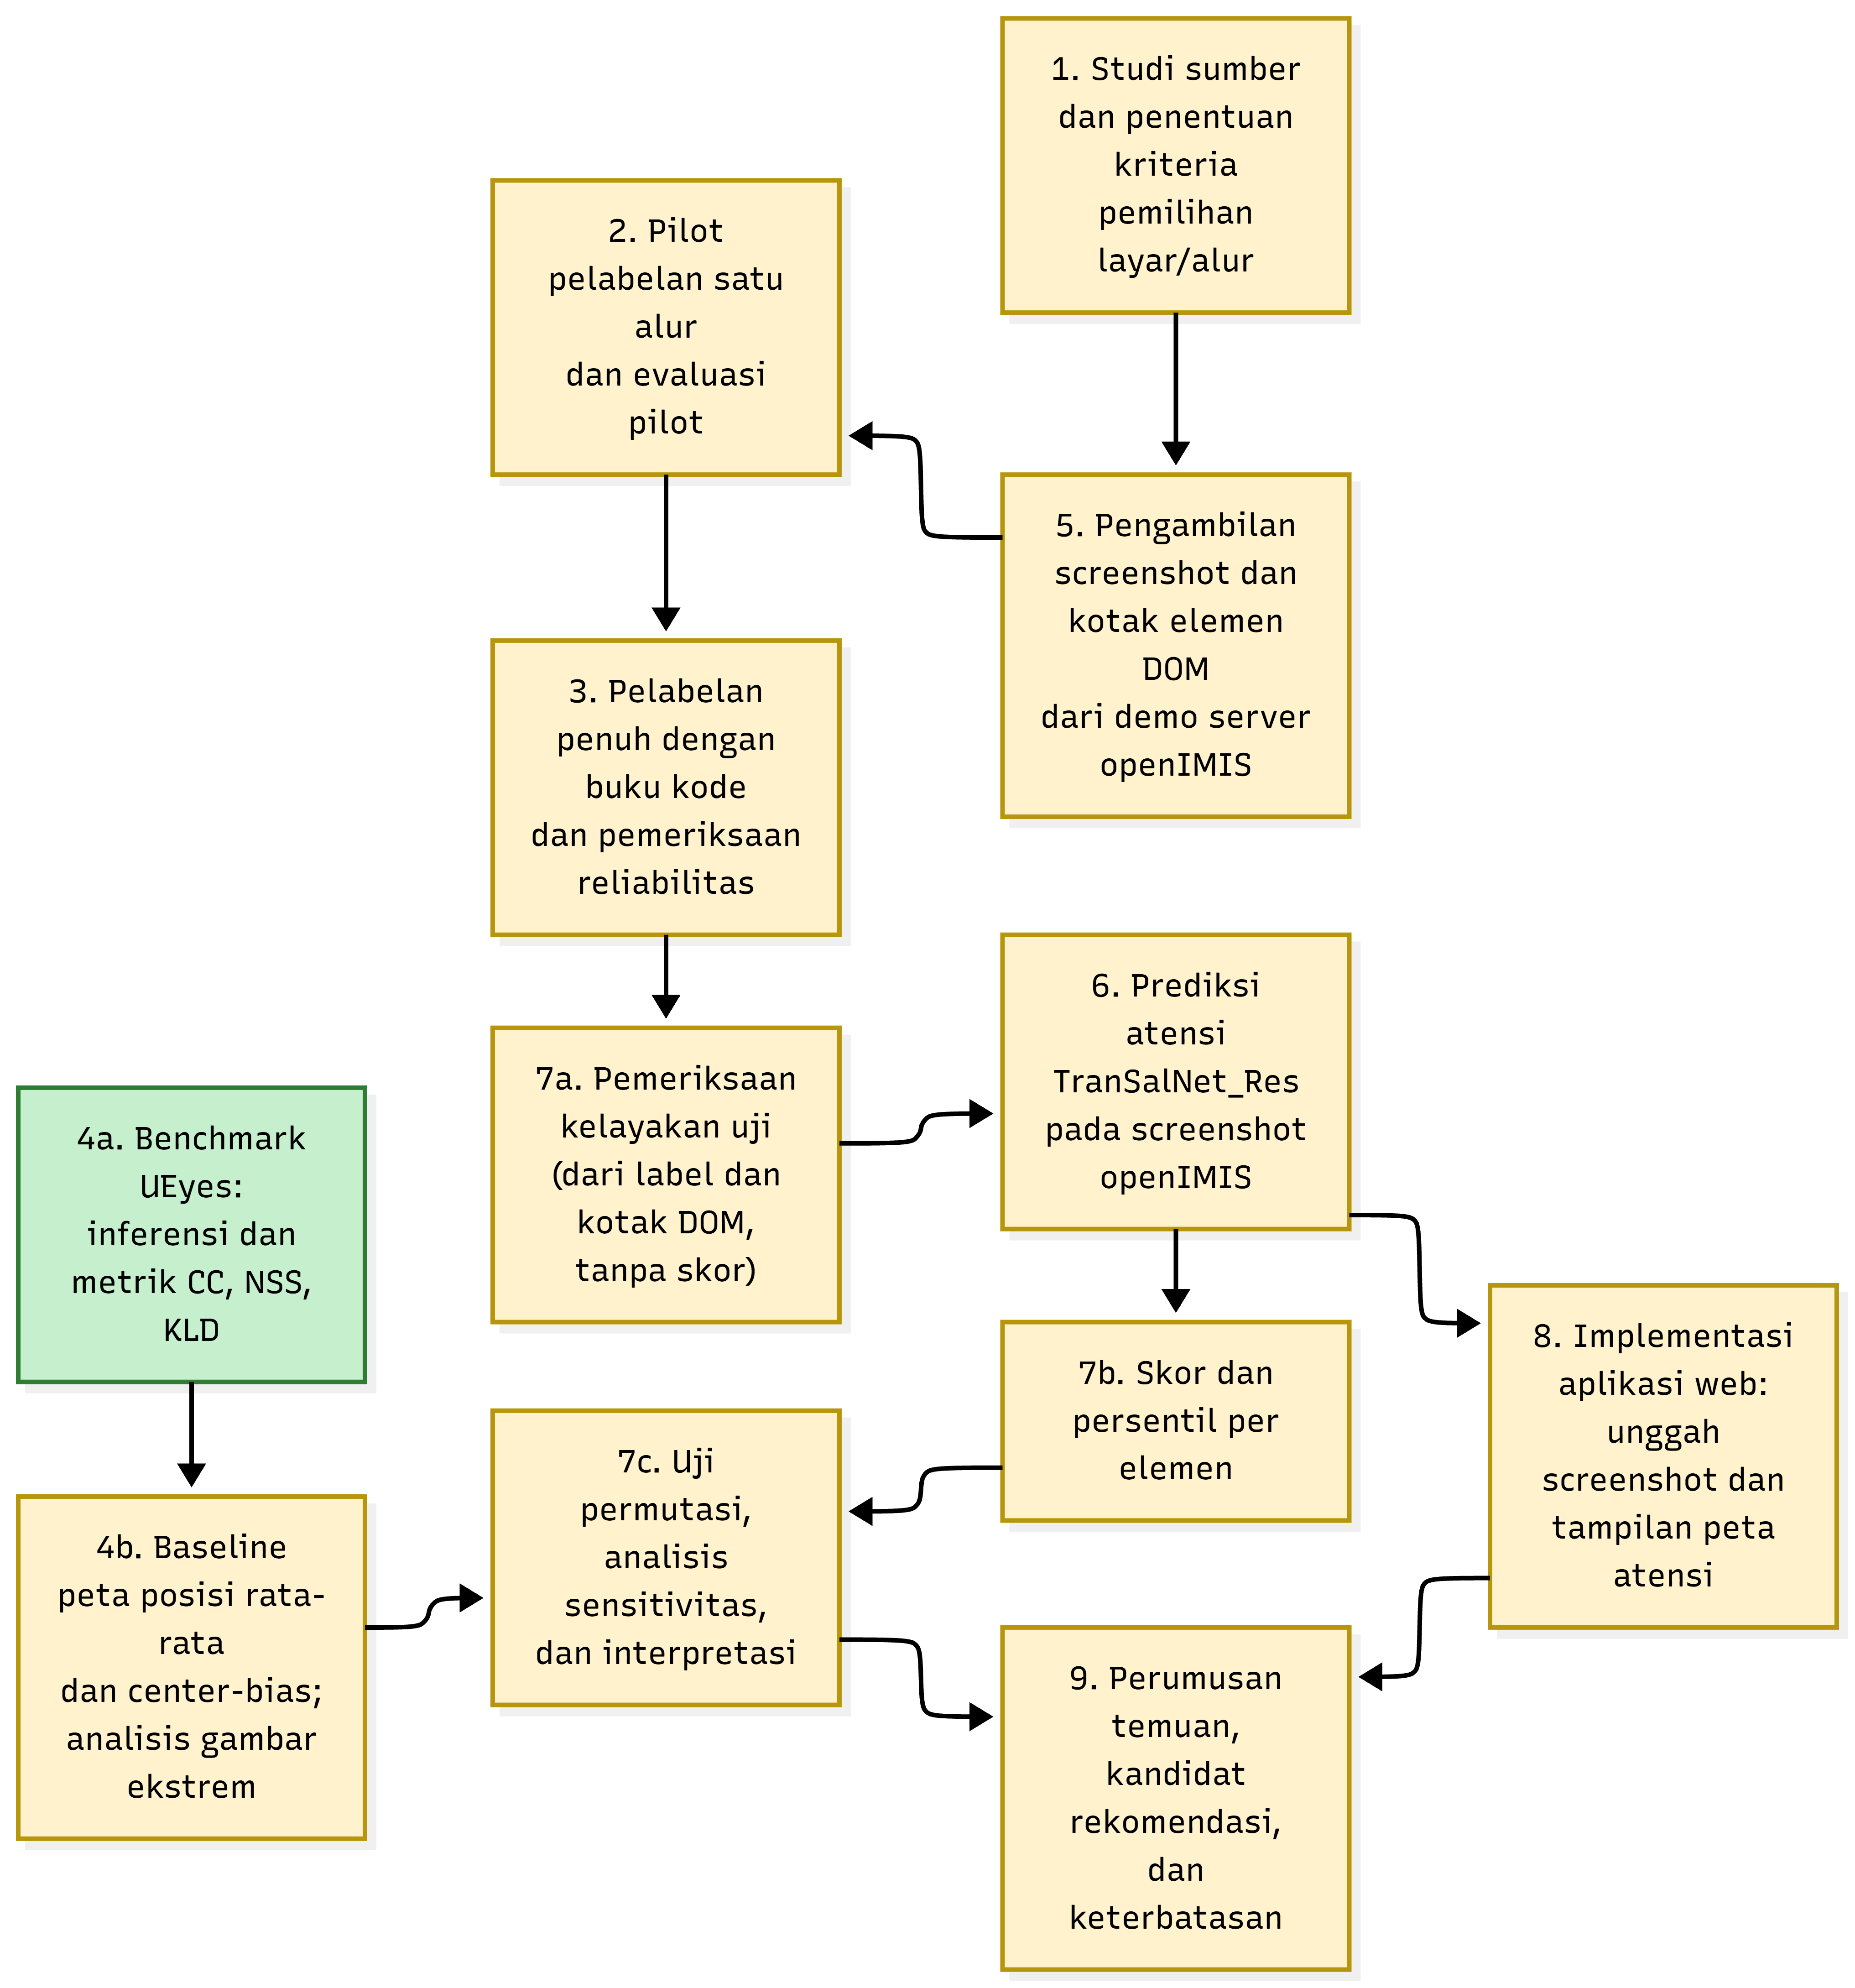
\includegraphics[width=\textwidth,height=0.85\textheight,keepaspectratio]{figures/bagan-alir}
  \caption{Bagan alir penelitian (hijau: telah dilaksanakan; kuning: akan dikerjakan)}
  \label{fig:bagan-alir}
\end{figure}

Gambar 3.1 menunjukkan urutan dan ketergantungan antartahap. Secara garis besar, tahapan terbagi menjadi empat kelompok: penyiapan data dan pelabelan (Tahap 1, 2, 3, dan 5), pengukuran kredibilitas model pada UEyes (Tahap 4), prediksi dan analisis pada antarmuka openIMIS (Tahap 6 dan 7), serta perumusan temuan (Tahap 8). Tahap 7 dipecah menjadi tiga langkah berurutan, yaitu pemeriksaan kelayakan uji, perhitungan skor, dan uji permutasi beserta analisis lanjutannya, karena mode analisis harus ditetapkan sebelum skor dihitung. Keluaran setiap tahap beserta indikator capaiannya yang terukur dirinci pada Tabel 3.1, dan indikator tersebut menjadi acuan untuk menilai keberhasilan setiap tahap.

\begin{longtable}{>{\raggedright\arraybackslash}p{0.20\textwidth}>{\raggedright\arraybackslash}p{0.24\textwidth}>{\raggedright\arraybackslash}p{0.46\textwidth}}
\caption{Tahapan penelitian, keluaran, dan indikator capaian}
\label{tab:tahapan}\\
\hline
\textbf{Tahap} & \textbf{Keluaran} & \textbf{Indikator capaian (terukur)} \\
\hline
\endfirsthead
\multicolumn{3}{l}{\emph{Tabel~\ref{tab:tahapan} (lanjutan)}}\\
\hline
\textbf{Tahap} & \textbf{Keluaran} & \textbf{Indikator capaian (terukur)} \\
\hline
\endhead
\hline
\endfoot
1. Studi sumber dan kriteria pemilihan layar/alur & Daftar sumber dan kriteria pemilihan & Setiap sumber tercatat lengkap (URL, tanggal terbit, tanggal akses, ciri versi antarmuka) \\
\hline
2. Pilot pelabelan & Buku kode mini dan evaluasi pilot & Setiap kriteria evaluasi pilot dinilai terhadap ambang pada Tabel~\ref{tab:evaluasi-pilot} dan keputusannya didokumentasikan; $\kappa$, $p_o$, PA, daftar elemen yang berubah label, dan kesepakatan per kriteria dilaporkan \\
\hline
3. Pelabelan penuh & Buku kode final dan tabel label elemen & Setiap elemen berlabel memiliki minimal dua sumber berbeda yang tercatat; label final seluruh elemen tersedia beserta versi buku kode yang dipakai \\
\hline
4. \emph{Benchmark} UEyes & Nilai CC, NSS, KLD per kategori dan \emph{baseline} & Ketiga metrik dilaporkan (rerata dan simpangan baku) per kategori desktop dan web bersama \emph{baseline} peta posisi rata-rata manusia (\emph{leave-one-out}) dan \emph{center-bias} (tiga nilai $\sigma$) pada gambar yang sama, disertai rerata selisih per gambar dan proporsi gambar tempat model unggul; gambar dengan skor ekstrem diperiksa \\
\hline
5. Pengambilan data openIMIS & Pasangan \emph{screenshot} dan berkas kotak elemen beserta metadata & Setiap \emph{screenshot} berpasangan dengan berkas kotak dan metadata (tanggal akses, ukuran \emph{viewport}, keadaan layar) \\
\hline
6. Prediksi atensi & Peta atensi & Peta dihasilkan untuk seluruh \emph{screenshot} dengan prapemrosesan identik dengan \emph{benchmark} \\
\hline
7. Kelayakan uji, skor, dan analisis & Laporan kelayakan uji, skor, persentil, nilai-p permutasi, hasil analisis sensitivitas (melalui skrip analisis) & Laporan kelayakan uji (jumlah kelompok informatif, total susunan, nilai-p minimum) disusun sebelum skor dihitung; persentil seluruh elemen berlabel dan sebaran per elemen dilaporkan, beserta jumlah elemen berlabel dan $T$ per layar; nilai-p eksak dilaporkan terhadap $\alpha = 0{,}05$ bila syarat kelayakan terpenuhi; luas kotak elemen berlabel dan pembanding dilaporkan per layar (median dan rasio); hasil analisis sensitivitas dengan pembanding A dan status ketahanan kesimpulan dilaporkan; hasil pemilahan peran posisi dan lembar telaah kualitatif untuk seluruh elemen terpilih tersedia \\
\hline
8. Perumusan temuan & Temuan, kandidat rekomendasi, keterbatasan & Setiap temuan disertai tingkat kekuatan klaim (kuat, terbatas, atau indikatif), ukuran ketidakpastian, dan keterbatasannya; tidak ada klaim tentang perilaku pengguna; setiap kandidat rekomendasi memuat elemen, bukti, arah perbaikan, dan pernyataan perlu diuji dengan pengguna, dengan elemen berkriteria K3 diprioritaskan \\
\end{longtable}

% =====================================================================
\section{Data}
\label{sec:data}

\subsection{Dataset UEyes (\emph{Benchmark})}
\label{subsec:ueyes}

UEyes \citep{jiang2023ueyes} adalah dataset \emph{eye-tracking} antarmuka digital yang terdiri atas 1.980 tangkapan layar pada empat kategori (laman web, desktop, \emph{mobile}, dan poster), dikumpulkan dari 62 partisipan menggunakan \emph{eye-tracker} Gazepoint GP3 60~Hz, dengan peta \emph{saliency} pada durasi 1, 3, dan 7 detik. Penelitian ini memakai dua kategori yang paling dekat secara struktural dengan openIMIS, yaitu desktop dan web, dengan acuan berupa \emph{heatmap} dan \emph{fixation map} berdurasi 7 detik. Durasi 7 detik dipilih karena merupakan durasi pengamatan terpanjang sehingga mencerminkan eksplorasi yang paling menyeluruh. Perlu dicatat bahwa UEyes dikumpulkan tanpa tugas spesifik (\emph{free-viewing}) \citep{jiang2023ueyes}, sehingga kesesuaiannya dengan perilaku \emph{task-driven} pada openIMIS tidak dapat diasumsikan.

% CATATAN [CEK]: paper UEyes melaporkan 495 gambar per kategori. Jelaskan penyebab
% 482 gambar pada kategori desktop sebelum Tabel 3.2 dipakai.
\begin{table}[H]
  \centering
  \caption{Subset UEyes yang digunakan untuk \emph{benchmark}}
  \label{tab:ueyes}
  \begin{tabular}{lr}
    \hline
    \textbf{Kategori} & \textbf{Jumlah gambar} \\
    \hline
    Desktop & 482 \\
    Web & 495 \\
    \hline
    Total & 977 \\
    \hline
  \end{tabular}
\end{table}

Tidak ada pembagian data latih, validasi, dan uji karena penelitian tidak melakukan pelatihan. Seluruh gambar pada Tabel~\ref{tab:ueyes} berfungsi sebagai data uji untuk mengukur kredibilitas umum model, bukan sebagai basis pelatihan untuk domain openIMIS.

\subsection{Data Antarmuka openIMIS}
\label{subsec:data-openimis}

Data antarmuka berupa tangkapan layar yang diambil dari server demo resmi openIMIS pada layar dan alur tugas yang dipilih berdasarkan kriteria berikut:
\begin{enumerate}
  \item alur tugas tercakup pada minimal dua sumber berbeda (mis.\ webinar dan dokumentasi resmi), sehingga pelabelan dengan aturan dua sumber dapat dilakukan;
  \item layar yang bersangkutan dapat dibuka pada server demo saat pengambilan data;
  \item layar memuat elemen formulir yang kotaknya dapat diekstraksi dari DOM;
  \item direncanakan tiga alur tugas dari empat proses yang didemonstrasikan pada Sesi~4 (pendaftaran, penelusuran, klaim, pembaruan), dengan minimum dua alur dan minimal tiga layar secara keseluruhan.
  % CATATAN: butir 4 usulan, menunggu persetujuan pembimbing.
\end{enumerate}

Protokol pengambilan dibakukan agar tangkapan layar dan kotak elemen selaras: (a)~setiap layar diambil pada posisi gulir paling atas (\emph{viewport} awal), karena pengguna pertama kali melihat layar dari posisi tersebut; (b)~ukuran jendela ditetapkan $1920 \times 1080$ piksel CSS dengan \emph{zoom} 100\% dan \emph{device pixel ratio} 1 melalui mode perangkat pada \emph{DevTools}, dan dicatat sebagai metadata; (c)~kolom dibiarkan dalam keadaan kosong, karena label kolom berubah posisi setelah diisi; (d)~tangkapan layar diambil dengan fitur \emph{capture screenshot} peramban pada sesi yang sama dengan ekstraksi kotak; dan (e)~tanggal akses, ukuran \emph{viewport}, dan ciri versi antarmuka dicatat sebagai metadata. Pengambilan awal pada layar Family/Group (\emph{viewport} $2573 \times 1385$ piksel) bersifat uji coba teknis dan diulang dengan pengaturan baku di atas.

Elemen yang berada di luar \emph{viewport} awal tidak dianalisis. Hal ini dinyatakan sebagai batasan penelitian.

\subsection{Sumber Pelabelan}
\label{subsec:sumber}

Sumber pelabelan terdiri atas (1)~video webinar pelatihan proses openIMIS tahun 2020, khususnya Sesi~4 yang diselenggarakan pada 13 Mei 2020 dan mendemonstrasikan proses (pendaftaran peserta, penelusuran informasi peserta, entri klaim dan peninjauan medis, serta pembaruan keanggotaan), (2)~dokumentasi resmi dan wiki openIMIS, dan (3)~video demonstrasi fitur openIMIS tahun 2026. Daftar sesi pelatihan beserta tautan rekamannya tersedia pada halaman wiki \emph{openIMIS online training} \citep{openimis2026}.

\begin{table}[H]
  \centering
  \caption{Atribut yang dicatat untuk setiap sumber}
  \label{tab:atribut-sumber}
  \begin{tabularx}{\textwidth}{>{\raggedright\arraybackslash}p{0.36\textwidth}>{\raggedright\arraybackslash}X}
    \hline
    \textbf{Atribut} & \textbf{Keterangan} \\
    \hline
    ID sumber & Kode unik (mis.\ S01) \\
    Jenis & Webinar, dokumentasi/wiki, atau video demo \\
    Judul dan URL & Identitas sumber \\
    Tanggal terbit/unggah dan tanggal akses & Untuk keterlacakan \\
    Versi/ciri antarmuka yang tampil & Nomor versi bila disebut, atau ciri tampilan \\
    Modul/alur yang dicakup & Menentukan sumber mana yang dapat mendukung label suatu elemen \\
    \hline
  \end{tabularx}
\end{table}

Sumber berasal dari versi antarmuka yang berbeda dengan server demo pada saat pengambilan data, dan nomor versi tidak selalu disebutkan. Pemetaan elemen dilakukan berdasarkan fungsinya, bukan posisi piksel, dan perbedaan versi dinyatakan sebagai keterbatasan.

\subsection{Kotak Elemen dari DOM}
\label{subsec:kotak-dom}

Posisi dan ukuran setiap elemen diperoleh dari \emph{Document Object Model} (DOM) halaman, yaitu struktur internal yang dibangun peramban untuk setiap elemen yang ditampilkan. Posisi dan ukuran kotak elemen relatif terhadap \emph{viewport} dapat dibaca melalui metode \texttt{getBoundingClientRect()} yang didefinisikan pada CSSOM View Module \citep{pieters2013cssom}. Pemodelan atensi pada tingkat elemen laman web juga pernah ditempuh oleh \citet{buscher2009what}. Untuk setiap elemen dicatat label teks, jenis, status wajib isi, status keterlihatan, serta posisi dan ukuran kotak dalam piksel gambar.

\begin{table}[H]
  \centering
  \caption{Contoh keluaran ekstraksi kotak elemen pada layar Family/Group (cuplikan uji coba awal; \emph{viewport} $2573 \times 1385$ piksel)}
  \label{tab:contoh-dom}
  \begin{tabular}{llcrrrr}
    \hline
    \textbf{Label} & \textbf{Jenis} & \textbf{Wajib} & \textbf{x} & \textbf{y} & \textbf{Lebar} & \textbf{Tinggi} \\
    \hline
    Region * & \emph{dropdown} & ya & 58 & 287 & 570 & 63 \\
    Confirmation No. & teks/lainnya & tidak & 848 & 374 & 564 & 63 \\
    Insurance No. * & teks/lainnya & ya & 61 & 624 & 761 & 63 \\
    \hline
  \end{tabular}
\end{table}

Kolom ``Jenis'' dihasilkan otomatis dan diperiksa secara visual; klasifikasi yang keliru dikoreksi secara manual dan koreksinya dicatat.

% =====================================================================
\section{Rancangan Metode}
\label{sec:rancangan-metode}

\subsection{Model Prediksi Atensi Visual}
\label{subsec:model}

Model yang digunakan adalah TranSalNet\_Res \citep{lou2022transalnet}, yaitu model yang menggabungkan \emph{encoder} CNN berbasis ResNet-50 dengan \emph{encoder Transformer}, dengan bobot pra-latih yang dilatih pada dataset SALICON \citep{jiang2023ueyes}. SALICON berisi data pengamatan bebas (\emph{free-viewing}) yang dikumpulkan dengan paradigma kontingen-\emph{mouse} pada citra MS COCO \citep{jiang2023ueyes}, bukan pada antarmuka digital, sehingga terdapat pergeseran domain antara data pelatihan model dan objek studi penelitian ini. Bobot model tidak diubah. Prapemrosesan bawaan TranSalNet mengubah ukuran gambar agar muat pada $384 \times 288$ piksel dengan mempertahankan rasio aspek (area sisa diisi \emph{padding}), lalu nilai piksel dinormalisasi ke rentang $[0, 1]$. Peta prediksi dikembalikan ke ukuran gambar asli dengan membuang \emph{padding}, kemudian dikonversi ke 8-bit. Prapemrosesan yang sama digunakan baik pada \emph{benchmark} UEyes maupun pada \emph{screenshot} openIMIS. Peta 8-bit dipakai baik untuk \emph{benchmark} maupun untuk perhitungan skor per elemen agar pemrosesan identik; pembulatan ke 256 tingkat berdampak dapat diabaikan karena skor elemen merupakan rerata banyak piksel di dalam kotak, dan nilai kembar ditangani oleh peringkat tengah pada Persamaan~\eqref{eq:persentil}.

Karena peta prediksi dikembalikan ke ukuran asli, koordinat kotak dari DOM dapat dipakai langsung pada peta. Namun resolusi efektif informasi atensi jauh lebih rendah daripada resolusi \emph{screenshot} (\emph{screenshot} $1920 \times 1080$ piksel diperkecil dengan faktor 0,2 menjadi $384 \times 216$ piksel pada ruang model, lalu diberi \emph{padding} hingga $384 \times 288$), sehingga elemen yang kecil diwakili oleh sedikit piksel; misalnya, kolom formulir setinggi 63 piksel hanya diwakili sekitar 13 piksel pada ruang model. Hal ini dicatat sebagai keterbatasan.

\subsection{Pelabelan Elemen Informasi Utama}
\label{subsec:pelabelan}

\textbf{Definisi operasional.} Elemen informasi utama adalah elemen antarmuka yang secara konsisten diperlakukan oleh sumber resmi (dokumentasi, materi pelatihan, video demonstrasi) sebagai pusat pelaksanaan suatu langkah proses administratif, yang didukung oleh minimal dua sumber berbeda, dan yang memenuhi minimal dua kriteria pada Tabel~\ref{tab:kriteria}. Kriteria dihitung secara gabungan lintas sumber, sehingga K1 yang ditemukan pada satu sumber dan K2 pada sumber lain dihitung sebagai dua kriteria; K4 yang diperoleh dari DOM turut dihitung sebagai kriteria, tetapi tidak dihitung sebagai sumber, sehingga syarat dua sumber tetap harus dipenuhi oleh bukti dari dokumentasi, materi pelatihan, atau video demonstrasi. Apabila pilot tidak mencapai jumlah elemen berlabel pada Tabel~\ref{tab:evaluasi-pilot}, nilai ini diturunkan menjadi satu kriteria dan perubahan tersebut dicatat.
% CATATAN: penurunan menjadi satu kriteria adalah usulan, menunggu persetujuan pembimbing.

\begin{table}[H]
  \centering
  \caption{Kriteria pelabelan}
  \label{tab:kriteria}
  \begin{tabularx}{\textwidth}{>{\raggedright\arraybackslash}p{0.07\textwidth}>{\raggedright\arraybackslash}p{0.18\textwidth}>{\raggedright\arraybackslash}X>{\raggedright\arraybackslash}p{0.26\textwidth}}
    \hline
    \textbf{Kode} & \textbf{Kriteria} & \textbf{Definisi operasional} & \textbf{Cara verifikasi} \\
    \hline
    K1 & Dipakai pada langkah inti alur & Elemen diisi, dibaca, atau diklik pada langkah yang oleh sumber disebut sebagai bagian inti alur tugas & Catatan bukti jenis ``dipakai di demo'' atau ``disebut dokumentasi'' \\
    \hline
    K2 & Ditekankan eksplisit & Sumber menyatakan secara tegas bahwa elemen itu wajib, penting, atau perlu diperhatikan & Catatan bukti jenis ``ditekankan'' \\
    \hline
    K3 & Menentukan status atau keputusan & Nilai elemen menentukan status atau hasil proses & Catatan bukti yang menghubungkan nilai elemen dengan hasil proses \\
    \hline
    K4 & Kolom wajib isi pada antarmuka & Elemen memiliki atribut wajib isi pada DOM & Otomatis dari data ekstraksi DOM; tidak dihitung sebagai sumber \\
    \hline
  \end{tabularx}
\end{table}

\textbf{Prosedur.} Pelabelan dilakukan oleh satu pelabel (peneliti) menggunakan buku kode terdokumentasi dengan langkah berikut: (1)~mendaftar sumber; (2)~memecah sumber menjadi langkah tugas dan mencatat elemen yang dipakai atau ditekankan beserta waktu atau bagian dokumen; (3)~menerapkan kriteria Tabel~\ref{tab:kriteria}; (4)~memberi label pada elemen yang didukung minimal dua sumber berbeda dan memenuhi minimal dua kriteria pada Tabel~\ref{tab:kriteria}; (5)~memetakan elemen pada sumber ke elemen pada hasil ekstraksi DOM berdasarkan fungsi dan teks labelnya, dan mencatat kode penyebab untuk elemen yang tidak dapat dipetakan, yaitu V (perbedaan versi: diganti nama, dipindah, digabung, atau dihapus), P (berada di luar \emph{viewport} awal), S (tidak tertangkap selektor, mis.\ tombol atau kotak pencarian), K (hanya muncul setelah interaksi), atau N (sumber merujuk tindakan atau konsep, bukan elemen antarmuka tertentu); dan (6)~mencatat status perbedaan versi untuk setiap elemen. Bukti dicatat dengan kata-kata peneliti sendiri secara ringkas, bukan salinan transkrip. Sebelum sesi pelabelan pertama, \emph{screenshot} dan kotak elemen DOM untuk seluruh layar alur pilot diambil terlebih dahulu (Subbab~\ref{subsec:data-openimis} dan~\ref{subsec:ekstraksi-dom}), sehingga lembar kerja pelabelan dapat disusun dengan satu baris untuk setiap elemen DOM dan kedua sesi menilai daftar elemen yang sama pada versi antarmuka yang sama.

\textbf{Pilot dan evaluasi pilot.} Sebelum pelabelan penuh, dilakukan pilot pada satu alur tugas yang mencakup seluruh layar pada alur tersebut. Hasil pilot dievaluasi dengan kriteria pada Tabel~\ref{tab:evaluasi-pilot}, yang ditetapkan sebelum pilot dijalankan agar penilaian tidak dipengaruhi hasil.

% CATATAN: seluruh ambang pada Tabel 3.6 adalah usulan, menunggu persetujuan pembimbing.
% CATATAN [CEK]: cocokkan rumus kesepakatan positif (PA) dengan makalah Cicchetti dan
% Feinstein (1990) sebelum dikutip.
\begin{longtable}{>{\raggedright\arraybackslash}p{0.17\textwidth}>{\raggedright\arraybackslash}p{0.27\textwidth}>{\raggedright\arraybackslash}p{0.46\textwidth}}
\caption{Kriteria evaluasi pilot dan penyesuaian prosedur}
\label{tab:evaluasi-pilot}\\
\hline
\textbf{Pertanyaan} & \textbf{Lanjut tanpa penyesuaian bila} & \textbf{Tindakan bila tidak terpenuhi} \\
\hline
\endfirsthead
\multicolumn{3}{l}{\emph{Tabel~\ref{tab:evaluasi-pilot} (lanjutan)}}\\
\hline
\textbf{Pertanyaan} & \textbf{Lanjut tanpa penyesuaian bila} & \textbf{Tindakan bila tidak terpenuhi} \\
\hline
\endhead
\hline
\endfoot
Apakah jumlah elemen berlabel cukup? & $\geq 10$ elemen berlabel pada alur pilot (diturunkan dari target total $\geq 30$ elemen pada tiga alur) & Dilakukan berurutan dan berhenti begitu ambang tercapai: (1)~tambah layar atau alur pada pilot; (2)~turunkan syarat dari minimal dua kriteria menjadi minimal satu kriteria; (3)~bila masih kurang, definisi elemen informasi utama diganti dengan properti dari DOM (mis.\ kolom wajib isi), hanya dengan persetujuan pembimbing karena mengubah pertanyaan penelitian. Setiap perubahan dicatat beserta alasannya \\
\hline
Apakah kriteria diterapkan konsisten? & Kappa kode-ulang $\geq 0{,}67$, dihitung pada seluruh elemen hasil ekstraksi DOM pada layar-layar alur pilot & Tentukan dulu penyebabnya. (a)~Bila $p_o \geq 0{,}85$ dan kesepakatan positif PA $\geq 0{,}80$, kappa rendah dianggap akibat sedikitnya elemen berlabel (paradoks prevalensi), bukan inkonsistensi; buku kode tidak direvisi, dan $p_o$, $\kappa$, PA, serta elemen yang berubah label dilaporkan. (b)~Bila tidak, elemen yang berubah label ditelaah untuk menemukan kriteria yang ambigu, definisi kriteria dipertajam dan diberi contoh kasus, lalu pengodean ulang dilakukan \\
\hline
Apakah pemetaan ke layar berhasil? & $\geq 80\%$ elemen yang lolos aturan dua sumber dapat dipetakan ke elemen DOM saat ini; elemen berkode P, S, dan N tidak dihitung karena berada di luar lingkup sejak awal & Dilakukan berurutan: (1)~untuk layar yang pemetaannya buruk, tambahkan sumber yang versinya lebih dekat dengan server demo (mis.\ video demonstrasi 2026 atau dokumentasi terbaru), lalu ulangi pemetaan; (2)~bila masih di bawah ambang, keluarkan layar yang persentase pemetaannya sendiri di bawah 80\%, sedangkan alur tetap dipakai selama masih ada layar tersisa; (3)~periksa ulang ambang jumlah elemen berlabel pada baris pertama. Layar yang dikeluarkan dicatat beserta alasannya sebagai keterbatasan \\
\end{longtable}

\textbf{Reliabilitas.} Konsistensi keputusan diperiksa hanya pada alur pilot, melalui pengodean ulang oleh peneliti yang sama (\emph{intra-rater}). Sesi kedua dilaksanakan sekurang-kurangnya dua minggu setelah sesi pertama dan mengulang langkah (2) sampai (4) prosedur pelabelan: sumber ditonton dan dibaca ulang, bukti dicatat ulang, lalu kriteria diterapkan dan label diberikan. Daftar sumber (langkah 1) dipakai ulang karena tidak memuat penilaian, sedangkan pemetaan ke DOM (langkah 5) dinilai terpisah melalui ambang pemetaan pada Tabel~\ref{tab:evaluasi-pilot}. Sesi kedua memakai lembar kerja baru dengan urutan elemen diacak; lembar kerja sesi pertama disimpan terpisah dan baru dibuka setelah sesi kedua selesai. Kesepakatan dilaporkan sebagai proporsi kesepakatan dan koefisien kappa \citep{cohen1960coefficient,hallgren2012computing}:
\begin{equation}
  \kappa = \frac{p_o - p_e}{1 - p_e}
  \label{eq:kappa}
\end{equation}
dengan $p_o$ proporsi elemen yang diberi label sama pada kedua sesi dan $p_e$ proporsi kesepakatan yang diharapkan terjadi secara kebetulan, dihitung dari proporsi marginal kedua sesi. Satuan perhitungan adalah setiap elemen hasil ekstraksi DOM pada layar-layar alur pilot, sehingga kedua sesi menilai himpunan elemen yang sama; elemen tanpa bukti dari sumber dinilai tidak berlabel. Elemen dari sumber yang tidak dapat dipetakan ke DOM tidak termasuk dalam perhitungan kappa, tetapi diperhitungkan pada ambang pemetaan. Kappa dihitung pada label akhir (berlabel atau tidak berlabel), disertai daftar elemen yang berubah label dan proporsi kesepakatan per kriteria K1 sampai K3 secara deskriptif untuk menelusuri sumber ketidaksepakatan.

Ambang kesepakatan mengikuti batas bawah tentatif 0,67 (Krippendorff, 1980, dikutip dalam \citealp{hallgren2012computing}); Landis dan Koch (1977, dikutip dalam \citealp{hallgren2012computing}) menyebut rentang 0,61 sampai 0,80 sebagai kesepakatan substansial, dan kedua batas tersebut diperdebatkan \citep{hallgren2012computing}. Ambang 80\% pada pemetaan elemen merupakan pertimbangan peneliti, bukan standar baku; ambang ini dimaksudkan mengukur apakah perbedaan versi antara sumber dan server demo masih dapat diatasi melalui pemetaan berbasis fungsi, sehingga penyebutnya hanya mencakup elemen berkode V dan K selain elemen yang berhasil dipetakan. Jumlah elemen untuk setiap kode penyebab tetap dilaporkan, karena banyaknya elemen berkode P atau S menunjukkan batas cakupan penelitian; apabila banyak elemen calon utama berkode S, perluasan selektor (Subbab~\ref{subsec:ekstraksi-dom}) diputuskan sebelum pelabelan penuh. Kesepakatan yang tinggi hanya menunjukkan keterulangan keputusan, bukan kebenaran label, sehingga hasil pelabelan tetap dinyatakan eksploratif karena tidak ada validasi oleh pakar domain.

\textbf{Label final.} Label yang dipakai pada analisis diambil dari sesi terakhir yang menggunakan buku kode final. Elemen yang labelnya berbeda antar-sesi diputuskan ulang dengan membaca kembali sumbernya, dan alasannya dicatat pada buku kode. Alur pilot turut dianalisis bersama alur lainnya; apabila buku kode direvisi setelah pilot, label alur pilot diambil dari putaran pengodean yang menggunakan buku kode hasil revisi. Alur selain pilot dilabel satu kali menggunakan buku kode final.

\subsection{Ekstraksi Kotak Elemen dari DOM}
\label{subsec:ekstraksi-dom}

Kotak elemen diperoleh melalui skrip yang dijalankan pada konsol peramban dan bersifat hanya-baca. Satu elemen didefinisikan sebagai kontainer terluar komponen kolom formulir (\texttt{MuiFormControl-root}) atau kotak centang berlabel (\texttt{MuiFormControlLabel-root}), sehingga label dan isian kolom diperlakukan sebagai satu elemen. Elemen dengan ukuran nol dilewati, keterlihatan elemen diperiksa pada titik tengahnya, dan seluruh koordinat dikalikan dengan rasio piksel perangkat (\emph{device pixel ratio}) agar sesuai dengan piksel gambar. Kotak elemen dipotong (\emph{clip}) ke batas \emph{viewport}; elemen yang bagian terlihatnya kurang dari 50\% luas kotaknya dikeluarkan dari analisis dan dicatat. Ambang 50\% merupakan pertimbangan peneliti. Nama kelas yang dibangkitkan otomatis oleh pustaka (mis.\ berawalan \texttt{jss}) tidak digunakan karena dapat berubah antarversi \emph{build}. Kesesuaian pasangan \emph{screenshot} dan kotak diperiksa dengan membandingkan lebar dan tinggi gambar terhadap ukuran \emph{viewport} yang dicetak oleh skrip.

Skrip pada tahap ini hanya menangkap elemen kolom formulir. Jenis elemen lain (tabel, tombol, judul, menu) ditambahkan pada selektor apabila alur yang dipilih memuatnya.

\subsection{Perhitungan Skor \emph{Saliency} per Elemen}
\label{subsec:skor}

Perhitungan pada subbab ini dikerjakan oleh skrip analisis (\emph{notebook}) yang menerima peta prediksi dan berkas kotak elemen. Skrip ini merupakan instrumen penelitian. Peta prediksi $S$ untuk setiap \emph{screenshot} distandarkan menjadi $S_z$, dengan $\mu_S$ dan $\sigma_S$ masing-masing rerata dan simpangan baku seluruh piksel pada peta tersebut:
\begin{equation}
  S_z(x,y) = \frac{S(x,y) - \mu_S}{\sigma_S}
  \label{eq:standardisasi}
\end{equation}
Skor \emph{saliency} elemen $e$ dengan kotak $B_e$ adalah rerata nilai peta terstandarkan di dalam kotak:
\begin{equation}
  s_e = \frac{1}{|B_e|}\sum_{(x,y)\in B_e} S_z(x,y)
  \label{eq:skor}
\end{equation}

Standardisasi pada Persamaan~\eqref{eq:standardisasi} tidak mengubah $P_e$ maupun $T$, karena persentil hanya bergantung pada urutan skor di dalam satu layar. Standardisasi dipertahankan agar $s_e$ dapat dilaporkan dan dibandingkan secara deskriptif antarlayar, misalnya ``elemen X berada 1,5 simpangan baku di atas rerata layarnya''.

Skor tersebut dibandingkan dengan himpunan pembanding $C_e$ menggunakan persentil dengan penanganan nilai kembar melalui peringkat tengah:
\begin{equation}
  P_e = 100 \times \frac{\left|\{c\in C_e : s_c < s_e\}\right| + 0{,}5\,\left|\{c\in C_e : s_c = s_e\}\right|}{|C_e|}
  \label{eq:persentil}
\end{equation}

Nilai $P_e = 50$ berarti elemen $e$ tidak berbeda dari pembanding. Dua himpunan pembanding digunakan: \textbf{pembanding B (utama)}, yaitu seluruh elemen tidak berlabel pada layar yang sama, apa pun jenisnya, dan \textbf{pembanding A (analisis sensitivitas)}, yaitu elemen tidak berlabel dengan jenis yang sama pada layar yang sama (kolom isian dengan kolom isian, \emph{dropdown} dengan \emph{dropdown}). Elemen berlabel lain tidak dijadikan pembanding, karena pertanyaan penelitian membandingkan elemen berlabel dengan elemen tidak berlabel. Pembanding B dipakai sebagai ukuran utama karena pertanyaan penelitian menyangkut tingkat menonjolnya elemen informasi utama pada antarmuka sebagaimana adanya; jenis elemen merupakan bagian dari keputusan desain, sehingga pengaruhnya termasuk dalam fenomena yang diamati. Pembanding A menjawab pertanyaan yang lebih sempit, yaitu apakah perbedaan tetap ada setelah jenis elemen disamakan, sehingga dipakai untuk menilai sejauh mana hasil utama berkaitan dengan jenis elemen. Karena jenis elemen berkaitan dengan ukuran kotak, sedangkan skor rerata dalam kotak peka terhadap ukuran kotak, luas kotak elemen berlabel dan pembandingnya dilaporkan per layar dalam bentuk median luas kotak elemen berlabel, median luas kotak pembanding B, dan rasio keduanya.

Pada pembanding B, himpunan pembanding hanya kosong apabila seluruh elemen pada suatu layar berlabel; layar seperti ini tidak disertakan dalam analisis utama dan dilaporkan secara deskriptif. Pada analisis sensitivitas dengan pembanding A, elemen berlabel yang tidak memiliki pembanding sejenis ($|C_e| = 0$), yaitu elemen pada kelompok layar dan jenis yang seluruh anggotanya berlabel, dikeluarkan dari analisis tersebut. Label elemen tersebut tidak dapat berpindah pada pengacakan (Subbab~\ref{subsec:permutasi}), sehingga persentilnya bernilai tetap pada setiap permutasi dan akan menggeser pusat distribusi nol $T$ dari 50; selain itu, menghitungnya terhadap pembanding lain akan mencampur dua definisi pembanding dalam satu statistik. Elemen tersebut tetap tercakup dalam analisis utama dengan pembanding B. Apabila elemen yang dikeluarkan dari analisis pembanding A melebihi 20\% dari seluruh elemen berlabel, jenis elemen digabung menurut hierarki jenis yang ditetapkan sebelum pelabelan (mis.\ kolom teks dan \emph{dropdown} digabung menjadi ``kolom isian'') \textbf{[hierarki ditetapkan sebelum pelabelan]}. Keputusan ini diambil pada pemeriksaan kelayakan uji, yang hanya memakai data label dan DOM. Elemen dengan pembanding sedikit tidak dikeluarkan, tetapi $|C_e|$ pada kedua pembanding dilaporkan untuk setiap elemen. Ambang 20\% merupakan pertimbangan peneliti.

Pembanding seluruhnya berasal dari kotak DOM; kotak yang ditempatkan secara acak tidak digunakan karena sering jatuh pada area kosong yang cenderung bernilai rendah dan akan membiaskan hasil ke arah elemen berlabel.

% =====================================================================
\section{Rancangan Pengujian dan Analisis}
\label{sec:pengujian}

\subsection{Protokol Evaluasi \emph{Benchmark}}
\label{subsec:benchmark}

Kredibilitas umum model diukur dengan membandingkan peta prediksi $S$ terhadap acuan UEyes. Notasi: $G$ adalah peta acuan (\emph{heatmap}), $F$ adalah peta fiksasi biner (bernilai 1 pada piksel fiksasi), $N=\sum_i F_i$ jumlah piksel fiksasi, dan indeks $i$ mencakup seluruh piksel. Implementasi metrik diadaptasi dari kode evaluasi resmi UEyes \citep{jiang2023ueyes} dengan dua penyesuaian yang didokumentasikan: normalisasi peta acuan dikoreksi agar memakai nilai maksimum peta acuan itu sendiri, dan tipe \texttt{np.bool} yang sudah dihapus pada NumPy versi baru diganti dengan \texttt{bool} bawaan Python.

\emph{Correlation Coefficient} (CC) adalah korelasi Pearson antara peta prediksi dan peta acuan (nilai lebih tinggi lebih baik):
\begin{equation}
  \mathrm{CC} = \frac{\sum_i (S_i-\bar{S})(G_i-\bar{G})}{\sqrt{\sum_i (S_i-\bar{S})^2\;\sum_i (G_i-\bar{G})^2}}
  \label{eq:cc}
\end{equation}

\emph{Normalized Scanpath Saliency} (NSS) adalah rerata nilai peta prediksi terstandarkan pada lokasi fiksasi (nilai lebih tinggi lebih baik):
\begin{equation}
  \mathrm{NSS} = \frac{1}{N}\sum_i F_i\,\frac{S_i-\mu_S}{\sigma_S}
  \label{eq:nss}
\end{equation}
% CATATAN [CEK]: pastikan berkas yang dipakai sebagai F adalah fixmaps_7s, bukan
% heatmaps_7s. Kode UEyes membuat mask dengan astype(bool).

\emph{Kullback-Leibler Divergence} (KLD) mengukur divergensi dari distribusi peta prediksi terhadap distribusi peta acuan, keduanya dinormalisasi hingga berjumlah satu (nilai lebih rendah lebih baik):
\begin{equation}
  \mathrm{KLD} = \sum_i p_i \ln\frac{p_i}{q_i},\qquad p_i=\frac{S_i+\varepsilon}{\sum_j (S_j+\varepsilon)},\quad q_i=\frac{G_i+\varepsilon}{\sum_j (G_j+\varepsilon)}
  \label{eq:kld}
\end{equation}
dengan $\varepsilon$ adalah epsilon mesin tipe \emph{float32} ($\approx 1{,}19\times10^{-7}$) yang mencegah pembagian dengan nol. Arah perhitungan pada Persamaan~\eqref{eq:kld} mengikuti implementasi UEyes, yaitu dari peta prediksi terhadap peta acuan, sehingga penalti lebih besar dijatuhkan pada atensi yang diprediksi pada area yang tidak diperhatikan. Arah ini berbeda dengan konvensi Bylinskii et al.\ (2019), yang menghitung divergensi dari peta acuan terhadap peta prediksi, sehingga nilai KLD tidak dibandingkan langsung dengan penelitian lain tanpa memeriksa arahnya. Arah pada implementasi UEyes ditentukan dari pembacaan kode evaluasi resminya, yang memanggil fungsi \texttt{entropy} dengan peta prediksi sebagai argumen pertama.

Ketiga metrik dilaporkan sebagai rerata dan simpangan baku \textbf{per kategori} (desktop dan web), tidak digabung, dan perbedaan arah antarkategori dilaporkan tanpa penyesuaian. Sebagai konteks, metrik yang sama dihitung untuk dua \emph{baseline} yang tidak memanfaatkan isi gambar, pada gambar yang sama:
\begin{enumerate}
  \item \textbf{Peta posisi rata-rata manusia (\emph{baseline} utama).} Untuk setiap gambar, \emph{baseline} adalah rerata peta acuan $G$ seluruh gambar lain dalam kategori yang sama (\emph{leave-one-out}), sehingga peta acuan gambar yang dievaluasi tidak ikut membentuk \emph{baseline}-nya. Seluruh peta acuan terlebih dahulu diubah ke resolusi bersama \textbf{[ditetapkan; usulan rasio 16:9 mengikuti openIMIS]}, lalu \emph{baseline} dikembalikan ke ukuran gambar asli. \emph{Baseline} ini dipilih sebagai \emph{baseline} utama karena Jiang et al.\ (2023) melaporkan bahwa fiksasi pada antarmuka, termasuk kategori web dan desktop, terkonsentrasi di kuadran kiri atas dan bukan di tengah, sehingga Gaussian tengah merupakan pembanding yang lemah untuk data ini.
  \item \textbf{Peta terpusat (\emph{center-bias}, \emph{baseline} pelengkap).} Distribusi Gaussian dua dimensi di tengah gambar dengan sebaran $\sigma$ sebesar 0,25 dari lebar dan tinggi gambar, disertai analisis kepekaan pada $\sigma = 0{,}15$ dan $\sigma = 0{,}35$. \emph{Baseline} ini dipertahankan karena lazim dilaporkan dalam evaluasi \emph{saliency} \citep{bylinskii2019what}. Penetapan $\sigma$ merupakan keputusan desain, bukan nilai optimum empiris; apabila model unggul hanya pada sebagian nilai $\sigma$, hal tersebut dilaporkan.
\end{enumerate}

Untuk setiap \emph{baseline}, kategori, dan nilai $\sigma$ dilaporkan (a)~rerata selisih per gambar (model $-$ \emph{baseline}) untuk CC, NSS, dan KLD (untuk KLD, selisih negatif berarti model lebih baik), dan (b)~proporsi gambar tempat model mengungguli \emph{baseline}; keduanya bersifat deskriptif. Model dinyatakan mengungguli peta posisi rata-rata manusia pada suatu kategori apabila proporsi gambar tempat model unggul melebihi 50\% pada sekurang-kurangnya dua dari tiga metrik; ketentuan ini merupakan pertimbangan peneliti. Hasil perbandingan ini menentukan cara menafsirkan peta model pada openIMIS: apabila model mengungguli peta posisi pada kedua kategori, peta model ditafsirkan sebagai prediksi yang memuat informasi isi layar; apabila tidak pada salah satu atau kedua kategori, setiap temuan pada openIMIS diberi kualifikasi bahwa prediksi model pada data \emph{benchmark} tidak lebih baik daripada pola posisi umum, dan hasil pemilahan peran posisi (Subbab~\ref{subsec:sensitivitas}) menjadi acuan utama penafsiran. Gambar dengan skor terbaik dan terburuk pada setiap metrik diperiksa secara visual untuk mengidentifikasi pola kegagalan. Perbandingan dengan angka penelitian lain (mis.\ UIGaze dan UMSI pada UEyes) diperlakukan sebagai indikatif dan hanya dilakukan setelah kesebandingan protokol evaluasi diperiksa.

\subsection{Hipotesis, Satuan Analisis, dan Ukuran}
\label{subsec:hipotesis}

Hipotesis, ukuran, dan prosedur uji ditetapkan sebelum model dijalankan pada \emph{screenshot} openIMIS. Hipotesis bersifat dua arah karena penelitian tidak memiliki dasar untuk memprediksi arah selisih:
\begin{itemize}
  \item \textbf{H\textsubscript{0}:} elemen informasi utama tidak berbeda menonjolnya dalam peta atensi visual prediktif dibandingkan elemen tidak berlabel pada layar yang sama.
  \item \textbf{H\textsubscript{1}:} elemen informasi utama berbeda menonjolnya (lebih menonjol atau kurang menonjol).
\end{itemize}

Taraf signifikansi ditetapkan $\alpha = 0{,}05$ (dua sisi) sebelum analisis dijalankan. Nilai-p dilaporkan secara eksak, tidak hanya sebagai signifikan atau tidak signifikan.

Satuan analisis adalah elemen berlabel, yang bersarang dalam layar dan alur tugas. Karena elemen pada layar yang sama tidak independen, uji inferensial dilakukan satu kali secara gabungan atas seluruh layar, dengan pengacakan label dibatasi di dalam layar yang sama (Subbab~\ref{subsec:permutasi}). Hasil per layar dilaporkan secara deskriptif tanpa nilai-p, karena uji terpisah per layar memiliki daya yang sangat rendah dan menimbulkan masalah perbandingan berganda. Ukuran utama adalah persentil $P_e$ terhadap pembanding B; ukuran pendukung adalah persentil terhadap pembanding A.

\subsection{Uji Permutasi}
\label{subsec:permutasi}

Statistik uji adalah rerata persentil seluruh elemen berlabel:
\begin{equation}
  T = \frac{1}{n}\sum_{e=1}^{n} P_e
  \label{eq:statistik-t}
\end{equation}
dengan $n$ jumlah elemen berlabel. Distribusi di bawah H\textsubscript{0} dibangun dengan mengacak ulang label ``berlabel'' di antara elemen DOM pada layar yang sama, lintas jenis elemen (jumlah elemen berlabel per layar dipertahankan), sebanyak $K = 10.000$ kali dengan \emph{random seed} tetap yang dicantumkan pada skrip, lalu menghitung ulang $T$ pada setiap pengacakan. Karena himpunan pembanding $C_e$ didefinisikan sebagai elemen tidak berlabel, pada setiap pengacakan $C_e$ dan $P_e$ dihitung ulang sesuai susunan label yang baru, sehingga $T_{\text{obs}}$ dan setiap $T_k$ diperoleh dengan prosedur yang identik. Apabila jumlah susunan label yang mungkin tidak melebihi 10.000, seluruh susunan didaftar sehingga nilai-p bersifat eksak, yaitu proporsi susunan (termasuk susunan amatan) yang sama atau lebih ekstrem tanpa penambahan satu. Nilai-p dua sisi dihitung sebagai:
\begin{equation}
  p = \frac{1 + \left|\{k : |T_k - 50| \geq |T_{\text{obs}} - 50|\}\right|}{K+1}
  \label{eq:nilai-p}
\end{equation}

Penambahan satu pada pembilang dan penyebut dilakukan agar nilai-p tidak pernah bernilai nol ketika permutasi diambil secara acak \citep{phipson2010permutation}. Perbandingan $|T_k - 50| \geq |T_{\text{obs}} - 50|$ dilakukan dengan toleransi numerik kecil, sehingga susunan yang secara matematis sama ekstremnya dengan susunan amatan tetap terhitung meskipun berbeda akibat pembulatan bilangan desimal. Apabila pada cara pengacakan nilai-p berada pada rentang 0,045 sampai 0,055, uji diulang dengan $K = 100.000$ untuk mengurangi ketidakpastian akibat pengambilan acak, dan nilai-p dari ulangan tersebut yang dipakai; aturan ini ditetapkan sebelum analisis agar keputusan tidak bergantung pada pilihan \emph{seed}.

Selain $T$ dan $p$, dilaporkan sebaran persentil setiap elemen, karena rerata dapat menyembunyikan pola yang sangat berbeda (semua elemen berada di sekitar persentil 45 berbeda maknanya dengan separuh elemen di persentil 90 dan separuh di persentil 0). Karena $T$ memberi bobot yang sama pada setiap elemen, layar dengan elemen berlabel terbanyak berpengaruh paling besar terhadap $T$. Oleh sebab itu, jumlah elemen berlabel dan nilai $T$ untuk setiap layar turut dilaporkan secara deskriptif, dan kesimpulan gabungan diberi kualifikasi apabila arah hasil tidak konsisten antarlayar. Rumus $T$ tidak diubah setelah data dilihat.

\textbf{Pemeriksaan kelayakan uji.} Uji permutasi hanya dapat menghasilkan nilai-p pada kelipatan tertentu yang ditentukan oleh jumlah susunan label yang mungkin. Untuk kelompok pengacakan $g$ (layar pada analisis utama; layar dan jenis pada analisis sensitivitas dengan pembanding A) dengan $n_g$ elemen, $k_g$ di antaranya berlabel, jumlah susunan total adalah:
\begin{equation}
  M = \prod_{g} \binom{n_g}{k_g}
  \label{eq:susunan}
\end{equation}

Kelompok yang hanya berisi elemen berlabel atau hanya berisi elemen tidak berlabel memiliki satu susunan dan tidak menyumbang informasi pada distribusi nol; kelompok yang memuat keduanya disebut kelompok informatif. Bila $M$ kecil, nilai-p terkecil yang dapat dicapai, yaitu nilai-p apabila seluruh elemen berlabel menempati peringkat tertinggi pada kelompoknya, dapat melebihi $\alpha$, sehingga uji tidak mungkin menghasilkan kesimpulan signifikan berapa pun besar efeknya (mis.\ tiga kelompok yang masing-masing berisi tiga elemen dengan satu elemen berlabel menghasilkan $M = 27$ dan nilai-p minimum dua sisi $2/27 \approx 0{,}074$). Hanya terdapat dua susunan yang paling ekstrem, yaitu seluruh elemen berlabel menempati peringkat tertinggi pada setiap kelompok ($T = 100$) atau peringkat terendah ($T = 0$), sehingga nilai-p minimum yang dapat dicapai adalah:
\begin{equation}
  p_{\min} =
  \begin{cases}
    \dfrac{2}{M}, & M \leq 10.000 \text{ (enumerasi penuh)} \\[2mm]
    \dfrac{1}{K+1}, & M > 10.000 \text{ (pengacakan sebanyak } K\text{)}
  \end{cases}
  \label{eq:pmin}
\end{equation}

Karena itu, setelah pelabelan dan ekstraksi kotak DOM selesai dan sebelum skor \emph{saliency} dihitung, dilaporkan (a)~jumlah kelompok informatif, (b)~nilai $M$, dan (c)~nilai $p_{\min}$. Pemeriksaan ini hanya memakai data label dan DOM sehingga tidak dipengaruhi hasil. Untuk menjaga hal tersebut, peta atensi openIMIS tidak dibuka, divisualisasikan, atau diolah menjadi skor sebelum laporan kelayakan uji selesai dan mode analisis ditetapkan. Pemeriksaan ini dilakukan untuk analisis utama dan analisis sensitivitas. Pada tahap yang sama ditentukan elemen berlabel yang dikeluarkan dari analisis pembanding A karena tidak memiliki pembanding sejenis, beserta penerapan penggabungan jenis bila jumlahnya melebihi ambang (Subbab~\ref{subsec:skor}). Kelompok yang seluruh anggotanya berlabel tidak disertakan dalam perhitungan $T$.

Uji inferensial dijalankan hanya bila kedua syarat berikut terpenuhi pada analisis utama: (1)~$p_{\min}$ tidak melebihi $\alpha$; dan (2)~jumlah elemen berlabel sekurang-kurangnya 30 yang tersebar pada sekurang-kurangnya tiga layar. Bila salah satu syarat tidak terpenuhi, hasil dilaporkan secara deskriptif per elemen dan per layar tanpa kesimpulan inferensial. Mode analisis yang ditetapkan pada analisis utama berlaku pula bagi analisis pada Subbab~\ref{subsec:sensitivitas}. Analisis sensitivitas dengan pembanding A, yang berfungsi sebagai pemeriksaan arah, cukup memenuhi syarat (1) pada kelompok pengacakannya sendiri; bila jumlah elemennya berkurang akibat pengeluaran elemen tanpa pembanding sejenis, penurunan daya uji tersebut dinyatakan sebagai keterbatasan, dan bila syarat (1) tidak terpenuhi, analisis A dilaporkan secara deskriptif. Analisis pemilahan peran posisi memakai label dan kelompok pengacakan yang sama dengan analisis utama sehingga kelayakannya identik.

Ambang syarat (2) diusulkan berdasarkan simulasi daya uji permutasi pada struktur yang menyerupai layar Family/Group, yang menunjukkan daya sekitar 0,65 pada 27 elemen berlabel dan sekitar 0,87 pada 36 elemen untuk efek sedang-besar (rerata persentil sekitar 69); daya jauh lebih rendah untuk efek kecil, sehingga hasil tidak signifikan tidak diartikan sebagai ketiadaan efek. Tidak ditemukan bukti perbedaan tidak sama dengan bukti kesetaraan, terutama pada sampel kecil.
% CATATAN: ambang syarat (2) usulan, menunggu persetujuan pembimbing.
% CATATAN [CEK]: simulasi daya uji perlu dijalankan ulang dengan rancangan terbaru
% (pembanding B, pengacakan per layar, pembanding dihitung ulang per permutasi).

\subsection{Analisis Sensitivitas dan Kualitatif}
\label{subsec:sensitivitas}

Subbab ini memuat tiga pemeriksaan tambahan atas hasil uji utama (Subbab~\ref{subsec:permutasi}), diikuti aturan interpretasi.

\textbf{Analisis sensitivitas pembanding.} Analisis sensitivitas dilakukan dengan mengulang seluruh analisis menggunakan pembanding A, dengan prosedur yang sama seperti Subbab~\ref{subsec:permutasi} (pembanding dihitung ulang pada setiap pengacakan, uji gabungan, dan pemeriksaan kelayakan uji). Karena pembanding A hanya memuat elemen sejenis, pengacakan label pada analisis ini dibatasi di dalam kelompok layar dan jenis yang sama, dan elemen tanpa pembanding sejenis dikeluarkan (Subbab~\ref{subsec:skor}). Apabila analisis utama (pembanding B) menghasilkan perbedaan signifikan, ketahanan kesimpulan tersebut terhadap penyamaan jenis elemen diklasifikasikan berdasarkan hasil analisis sensitivitas (pembanding A):
\begin{enumerate}
  \item \textbf{bertahan}, apabila analisis A juga signifikan dengan arah yang sama; kesimpulan utama tidak dijelaskan oleh jenis atau ukuran elemen;
  \item \textbf{melemah}, apabila analisis A tidak signifikan tetapi $T_A$ berada pada sisi yang sama terhadap 50; sebagian hasil mungkin berkaitan dengan jenis atau ukuran elemen;
  \item \textbf{tidak bertahan}, apabila $T_A$ berada pada sisi yang berlawanan terhadap 50; kesimpulan utama kemungkinan besar terdorong oleh jenis atau ukuran elemen, dan hal ini dilaporkan sebagai temuan, bukan sebagai ketiadaan temuan.
\end{enumerate}
Apabila analisis utama tidak signifikan, klasifikasi ini tidak digunakan dan hasil analisis A dilaporkan sebagai informasi pelengkap. Apabila analisis A berada pada mode deskriptif, yang dilaporkan hanya posisi $T_A$ terhadap 50.

\textbf{Pemilahan peran posisi.} Letak elemen merupakan bagian dari keputusan desain yang juga memengaruhi atensi: elemen berlabel cenderung ditempatkan di bagian atas dan kiri layar, sedangkan fiksasi pada antarmuka dilaporkan terkonsentrasi di kuadran kiri atas, bukan di tengah \citep{jiang2023ueyes}. Untuk memilah apakah menonjolnya elemen berlabel terutama berasal dari tata letak atau juga dari tampilan visual elemen, analisis utama Subbab~\ref{subsec:permutasi} (skor, persentil terhadap pembanding B, dan uji permutasi) dijalankan ulang dengan \textbf{peta posisi rata-rata manusia} sebagai pengganti peta model pada \emph{screenshot} openIMIS yang sama, dengan kotak, pembanding, dan prosedur pengacakan yang sama. Peta ini adalah rerata seluruh peta acuan UEyes kategori desktop dan web (Subbab~\ref{subsec:benchmark}), diubah ke ukuran \emph{screenshot} openIMIS, sehingga hanya memuat pola posisi umum dan tidak memanfaatkan isi layar; \emph{leave-one-out} tidak diperlukan karena \emph{screenshot} openIMIS bukan bagian dari UEyes. Nilai $T$ dan nilai-p dari peta posisi dilaporkan berdampingan dengan hasil peta model, dan ditafsirkan sebagai berikut:
\begin{enumerate}
  \item apabila peta posisi saja menghasilkan perbedaan signifikan ($p \leq \alpha$) dengan arah yang sama dengan peta model, menonjolnya elemen berlabel ditafsirkan dapat dijelaskan oleh tata letak;
  \item apabila peta model menghasilkan perbedaan signifikan sedangkan peta posisi tidak, terdapat indikasi bahwa tampilan visual elemen (mis.\ kontras, ukuran, atau penekanan) turut berperan di luar pola posisi umum;
  \item apabila peta posisi menunjukkan elemen berlabel lebih menonjol secara signifikan, tetapi peta model menunjukkan elemen tersebut tidak berbeda atau kurang menonjol, elemen ditafsirkan berada pada letak yang strategis tetapi kalah menonjol secara visual, dan menjadi bahan utama kandidat rekomendasi.
\end{enumerate}

Selain penafsiran pada tingkat gabungan, setiap elemen berlabel dengan persentil terhadap peta posisi $P_{\text{posisi}} \geq 75$ dan persentil terhadap peta model $P_{\text{model}} \leq 25$ ditandai secara deskriptif sebagai elemen ``posisi strategis, tampilan kalah'', karena letaknya termasuk seperempat teratas menurut pola posisi umum tetapi tampilannya termasuk seperempat terbawah menurut model. Penandaan ini berlaku pada kedua mode analisis dan menjadi masukan bagi telaah kualitatif.

Pemilahan ini tidak dimaksudkan untuk membatalkan temuan, karena tata letak merupakan bagian dari desain antarmuka, melainkan untuk mengarahkan kandidat rekomendasi pada penempatan elemen atau pada gaya visualnya. Peta posisi berasal dari antarmuka umum, bukan openIMIS, dan perubahan ukuran dapat mendistorsi pola bila rasio aspek berbeda; keduanya dinyatakan sebagai keterbatasan.

\textbf{Telaah kualitatif.} Elemen yang ditelaah adalah elemen berlabel dengan persentil ekstrem terhadap pembanding B ($P_e \leq 25$ sebagai kandidat masalah desain dan $P_e \geq 75$ sebagai contoh pembanding yang menonjol), ditambah elemen bertanda ``posisi strategis, tampilan kalah''. Setiap elemen ditelaah dengan lembar telaah yang atributnya ditetapkan sebelum analisis, yaitu: (1)~luas kotak relatif terhadap median pembanding; (2)~posisi, berupa kuadran layar dan $P_{\text{posisi}}$; (3)~letak area paling panas di dalam kotak (pada teks label, pada isian, atau tidak ada); (4)~penekanan visual yang tampak (mis.\ huruf tebal, warna, tanda bintang, ikon); (5)~pesaing atensi, yaitu satu sampai dua elemen tidak berlabel dengan skor tertinggi pada layar yang sama; (6)~hipotesis penjelasan; dan (7)~arah kandidat rekomendasi, yaitu penempatan atau gaya visual, mengacu pada pemilahan peran posisi. Atribut (1), (2), dan (5) diperoleh dari keluaran skrip, atribut (3) dan (4) dari pengamatan visual, sedangkan atribut (6) dan (7) merupakan interpretasi peneliti. Seluruh isi lembar telaah dinyatakan sebagai hipotesis untuk pengujian lanjutan dengan pengguna, bukan sebagai kesimpulan.
% CATATAN: opsional, ditunda: pengukuran kontras label terhadap latar dengan rasio
% kontras luminans WCAG.

\textbf{Aturan interpretasi.} Interpretasi hasil selalu menimbang empat hal: besar selisih, ketidakpastian (nilai-p), sebaran antarelemen, dan konsistensi arah antarlayar, serta dibatasi pada atensi visual prediktif. Kekuatan setiap temuan dinyatakan dalam tiga tingkat: (1)~\textbf{kuat}, bila analisis inferensial menghasilkan perbedaan signifikan dengan status bertahan; (2)~\textbf{terbatas}, bila signifikan dengan status melemah atau tidak bertahan, sehingga perbedaan sebagian dapat berkaitan dengan jenis atau ukuran elemen; dan (3)~\textbf{indikatif}, bila analisis berada pada mode deskriptif atau tidak signifikan. Temuan dirumuskan dengan frasa ``menurut prediksi model'' atau ``atensi visual prediktif''; frasa yang menyatakan perilaku pengguna, seperti ``pengguna melihat'', ``pengguna mengabaikan'', atau ``elemen tidak terbaca'', tidak digunakan. Kualifikasi dari hasil \emph{benchmark} (Subbab~\ref{subsec:benchmark}) diterapkan pada seluruh tingkat.

\textbf{Kandidat rekomendasi.} Kandidat rekomendasi hanya diturunkan dari elemen pada lembar telaah kualitatif yang memiliki $P_e \leq 25$ terhadap pembanding B atau bertanda ``posisi strategis, tampilan kalah''. Setiap kandidat rekomendasi memuat: (a)~elemen dan layarnya; (b)~bukti, yaitu $P_{\text{model}}$, $P_{\text{posisi}}$, dan pesaing atensi; (c)~arah perbaikan, yaitu penempatan atau gaya visual; dan (d)~pernyataan bahwa rekomendasi perlu diuji dengan pengguna. Elemen yang memenuhi kriteria K3 (menentukan status atau keputusan; Tabel~\ref{tab:kriteria}) diprioritaskan, karena kurang menonjolnya elemen penentu keputusan dipandang paling berisiko bagi pelaksanaan proses administratif.

% =====================================================================
\section{Ancaman Validitas dan Keterbatasan}
\label{sec:validitas}

\begin{longtable}{>{\raggedright\arraybackslash}p{0.21\textwidth}>{\raggedright\arraybackslash}p{0.33\textwidth}>{\raggedright\arraybackslash}p{0.36\textwidth}}
\caption{Ancaman validitas dan mitigasi}
\label{tab:validitas}\\
\hline
\textbf{Ancaman} & \textbf{Penjelasan} & \textbf{Mitigasi} \\
\hline
\endfirsthead
\multicolumn{3}{l}{\emph{Tabel~\ref{tab:validitas} (lanjutan)}}\\
\hline
\textbf{Ancaman} & \textbf{Penjelasan} & \textbf{Mitigasi} \\
\hline
\endhead
\hline
\endfoot
Label bersumber dari penekanan sumber, bukan kebutuhan informasi pengguna & Label mencerminkan apa yang dijelaskan sumber, bukan apa yang berisiko jika terlewat & Kriteria tertulis, dua sumber berbeda, dinyatakan eksploratif \\
\hline
Pelabel tunggal dan tanpa validasi pakar & Subjektivitas tidak hilang & Buku kode, pengodean ulang, dan kappa \\
\hline
Perbedaan versi antarmuka & Sumber 2020, video 2026, dan server demo saat ini bisa berbeda & Pemetaan berdasarkan fungsi, log versi, status pemetaan per elemen \\
\hline
Model \emph{bottom-up} dan acuan \emph{free-viewing} & Hasil tidak mewakili atensi pengguna yang bertugas & Klaim dibatasi pada atensi visual prediktif \\
\hline
Resolusi efektif rendah & Elemen kecil diwakili sedikit piksel pada ruang model & Dicatat sebagai keterbatasan; elemen sangat kecil ditandai \\
\hline
Jumlah elemen berlabel sedikit atau susunan label terbatas & Daya uji rendah; nilai-p minimum yang dapat dicapai bisa melebihi $\alpha$ & Pemeriksaan kelayakan uji sebelum skor dihitung (nilai-p minimum, Persamaan~\eqref{eq:susunan} dan~\eqref{eq:pmin}) dan ambang minimum (30 elemen pada tiga layar); pelaporan deskriptif bila salah satu syarat tidak terpenuhi \\
\hline
Dominasi satu layar & Nilai $T$ dapat didominasi oleh layar yang memiliki elemen berlabel paling banyak, sehingga tidak mewakili seluruh layar secara seimbang & $T$ dan jumlah elemen berlabel dilaporkan per layar; kesimpulan gabungan diberi kualifikasi bila arah tidak konsisten antarlayar \\
\hline
Ukuran dan jenis elemen & Pembanding utama (B) mencakup semua jenis elemen; jenis elemen berkaitan dengan ukuran kotak, dan skor rerata dalam kotak peka terhadap ukuran, sehingga persentil dapat sebagian mencerminkan ukuran atau jenis elemen & Luas kotak elemen berlabel dan pembanding dilaporkan per layar; analisis sensitivitas dengan pembanding A (jenis sama); perbedaan arah antara kedua pembanding ditafsirkan sebagai indikasi peran jenis atau ukuran elemen \\
\hline
Peran posisi (tata letak) & Elemen berlabel terkonsentrasi di bagian atas dan kiri, sejalan dengan bias kiri-atas pada fiksasi antarmuka \citep{jiang2023ueyes}; tanpa pemilahan, tidak jelas apakah menonjolnya elemen berasal dari tata letak atau dari tampilan visual & Tidak dikendalikan secara statistik karena tata letak merupakan bagian dari desain; perannya dipilah dengan menjalankan ulang analisis utama, termasuk uji permutasi, memakai peta posisi rata-rata manusia dari UEyes (Subbab~\ref{subsec:sensitivitas}) \\
\hline
Definisi elemen mencakup label dan isian & Skor elemen mencampur atensi pada teks label (cenderung lebih menonjol) dan kotak isian kosong (cenderung redup), sehingga menonjolnya label tidak dapat dipisahkan dari isiannya & Dinyatakan sebagai keterbatasan; definisi dipertahankan karena label dan isian dipersepsi sebagai satu kesatuan elemen formulir (Subbab~\ref{subsec:ekstraksi-dom}) \\
\hline
Cakupan terbatas & \emph{Viewport} awal, kolom formulir, server demo & Dinyatakan sebagai batasan \\
\hline
Tidak ada validasi kuantitatif domain-spesifik & Akurasi model hanya diukur pada UEyes & Dinyatakan eksplisit sebagai keterbatasan \\
\end{longtable}
% CATATAN: tiga usulan terkait dominasi area navigasi openIMIS (ukur porsi atensi,
% sensitivitas masking, pengaman 8-bit) ditahan; lihat Pertanyaan 6 bahan bimbingan.

% =====================================================================
% BAB 4 JADWAL PENELITIAN
% Membutuhkan di preambul: \usepackage[table]{xcolor}, \usepackage{multirow},
% \usepackage{array}, \usepackage{float}.
% =====================================================================
\definecolor{ganttisi}{gray}{0.45}
\definecolor{ganttcadangan}{gray}{0.82}
\newcommand{\gantt}{\cellcolor{ganttisi}}
\newcommand{\ganttcadangan}{\cellcolor{ganttcadangan}}

\chapter{JADWAL PENELITIAN}
\label{chap:jadwal}

\section{Jadwal Penelitian}
\label{sec:jadwal}

Jadwal penelitian disusun berdasarkan tahapan pada Tabel~\ref{tab:tahapan} dan ketergantungan antartahap pada Gambar~\ref{fig:bagan-alir}, dengan acuan jadwal ujian proposal Program Studi S1 Ilmu Komputer periode Desember 2026 (batas pendaftaran 7 Desember 2026 dan pelaksanaan ujian 14--18 Desember 2026) serta target ujian skripsi pada Juni 2027. Jadwal disajikan dalam bentuk \emph{Gantt chart} berbasis bulan yang dibagi per minggu, yaitu Tabel~\ref{tab:jadwal-1} untuk November 2026 sampai Februari 2027 dan Tabel~\ref{tab:jadwal-2} untuk Maret sampai Juli 2027. Nomor pada nama kegiatan merujuk pada nomor tahap di Tabel~\ref{tab:tahapan}. Tahap 4a (inferensi dan perhitungan metrik pada benchmark UEyes) telah dilaksanakan sebelum periode jadwal ini (Gambar~\ref{fig:bagan-alir}), sehingga tidak dicantumkan.

Urutan kegiatan mengikuti empat ketentuan pada Bab 3: (1)~screenshot dan kotak elemen DOM untuk layar alur pilot diambil sebelum sesi pertama pilot pelabelan (Subbab~\ref{subsec:pelabelan}); (2)~sesi kedua pengodean ulang pada pilot dilaksanakan sekurang-kurangnya dua minggu setelah sesi pertama; (3)~skrip analisis disiapkan dan divalidasi selama jeda tersebut dan selama pelabelan penuh, sebelum dipakai pada data openIMIS; dan (4)~pemeriksaan kelayakan uji (Tahap 7a) diselesaikan sebelum peta atensi openIMIS dibuka dan diolah menjadi skor (Subbab~\ref{subsec:permutasi}).

% CATATAN: kalimat cakupan dua alur adalah usulan, menunggu persetujuan pembimbing.
Cadangan waktu dua minggu disediakan untuk satu putaran pengodean ulang apabila evaluasi pilot menghasilkan keputusan \emph{lanjut dengan penyesuaian} (Tabel~\ref{tab:evaluasi-pilot}). Apabila cadangan tersebut terpakai, pelabelan penuh dimulai paling lambat dua minggu kemudian, dan cakupannya disesuaikan ke batas minimum dua alur tugas (Subbab~\ref{subsec:data-openimis}) agar pemeriksaan kelayakan uji tetap dapat diselesaikan pada akhir Maret 2027. Jadwal ujian skripsi tahun 2027 belum diterbitkan, sehingga posisi pendaftaran dan ujian skripsi pada Tabel~\ref{tab:jadwal-2} mengikuti pola jadwal prodi periode Juni 2026, yaitu batas pendaftaran pada akhir bulan sebelumnya dan ujian pada minggu pertama bulan berjalan; jadwal disesuaikan setelah jadwal resmi diterbitkan.

Pada Tabel~\ref{tab:jadwal-1} dan Tabel~\ref{tab:jadwal-2}, sel berwarna gelap menunjukkan rencana kegiatan dan sel berwarna terang menunjukkan cadangan waktu.

\begin{table}[H]
  \centering
  \footnotesize
  \setlength{\tabcolsep}{1.5pt}
  \renewcommand{\arraystretch}{1.25}
  \caption{Jadwal penelitian November 2026 sampai Februari 2027}
  \label{tab:jadwal-1}
  \begin{tabular}{|>{\raggedright\arraybackslash}p{0.36\textwidth}|*{4}{>{\centering\arraybackslash}p{0.032\textwidth}}|*{4}{>{\centering\arraybackslash}p{0.032\textwidth}}|*{4}{>{\centering\arraybackslash}p{0.032\textwidth}}|*{4}{>{\centering\arraybackslash}p{0.032\textwidth}}|}
  \hline
  \multirow{2}{*}{\textbf{Kegiatan}} & \multicolumn{4}{c|}{\textbf{Nov 2026}} & \multicolumn{4}{c|}{\textbf{Des 2026}} & \multicolumn{4}{c|}{\textbf{Jan 2027}} & \multicolumn{4}{c|}{\textbf{Feb 2027}} \\
  \cline{2-17}
   & 1 & 2 & 3 & 4 & 1 & 2 & 3 & 4 & 1 & 2 & 3 & 4 & 1 & 2 & 3 & 4 \\
  \hline
  Finalisasi proposal dan bimbingan &  &  &  & \gantt & \gantt &  &  &  &  &  &  &  &  &  &  &  \\
  \hline
  Simulasi daya uji dengan rancangan terbaru &  &  &  & \gantt & \gantt &  &  &  &  &  &  &  &  &  &  &  \\
  \hline
  Pendaftaran ujian proposal &  &  &  &  & \gantt &  &  &  &  &  &  &  &  &  &  &  \\
  \hline
  Ujian proposal &  &  &  &  &  &  & \gantt &  &  &  &  &  &  &  &  &  \\
  \hline
  Revisi proposal &  &  &  &  &  &  &  & \gantt & \gantt &  &  &  &  &  &  &  \\
  \hline
  1. Studi sumber dan kriteria pemilihan layar/alur &  &  &  & \gantt & \gantt & \gantt & \gantt & \gantt &  &  &  &  &  &  &  &  \\
  \hline
  4b. Baseline benchmark dan analisis gambar ekstrem &  &  &  &  &  &  &  & \gantt & \gantt & \gantt & \gantt & \gantt &  &  &  &  \\
  \hline
  5. Pengambilan screenshot dan kotak elemen DOM &  &  &  &  &  &  &  & \gantt & \gantt & \gantt &  &  &  &  &  &  \\
  \hline
  2. Pilot pelabelan dan evaluasi pilot &  &  &  &  &  &  &  &  &  & \gantt & \gantt & \gantt & \gantt & \gantt &  &  \\
  \hline
  Cadangan satu putaran pengodean ulang pilot &  &  &  &  &  &  &  &  &  &  &  &  &  &  & \ganttcadangan & \ganttcadangan \\
  \hline
  3. Pelabelan penuh &  &  &  &  &  &  &  &  &  &  &  &  &  &  & \gantt & \gantt \\
  \hline
  Penyiapan dan validasi skrip analisis &  &  &  &  &  &  &  &  &  &  &  &  & \gantt & \gantt & \gantt & \gantt \\
  \hline
  \end{tabular}
\end{table}

\begin{table}[H]
  \centering
  \footnotesize
  \setlength{\tabcolsep}{1.5pt}
  \renewcommand{\arraystretch}{1.25}
  \caption{Jadwal penelitian Maret sampai Juli 2027}
  \label{tab:jadwal-2}
  \begin{tabular}{|>{\raggedright\arraybackslash}p{0.32\textwidth}|*{4}{>{\centering\arraybackslash}p{0.025\textwidth}}|*{4}{>{\centering\arraybackslash}p{0.025\textwidth}}|*{4}{>{\centering\arraybackslash}p{0.025\textwidth}}|*{4}{>{\centering\arraybackslash}p{0.025\textwidth}}|*{4}{>{\centering\arraybackslash}p{0.025\textwidth}}|}
  \hline
  \multirow{2}{*}{\textbf{Kegiatan}} & \multicolumn{4}{c|}{\textbf{Mar 2027}} & \multicolumn{4}{c|}{\textbf{Apr 2027}} & \multicolumn{4}{c|}{\textbf{Mei 2027}} & \multicolumn{4}{c|}{\textbf{Jun 2027}} & \multicolumn{4}{c|}{\textbf{Jul 2027}} \\
  \cline{2-21}
   & 1 & 2 & 3 & 4 & 1 & 2 & 3 & 4 & 1 & 2 & 3 & 4 & 1 & 2 & 3 & 4 & 1 & 2 & 3 & 4 \\
  \hline
  3. Pelabelan penuh & \gantt & \gantt & \gantt &  &  &  &  &  &  &  &  &  &  &  &  &  &  &  &  &  \\
  \hline
  Penyiapan dan validasi skrip analisis & \gantt & \gantt &  &  &  &  &  &  &  &  &  &  &  &  &  &  &  &  &  &  \\
  \hline
  7a. Pemeriksaan kelayakan uji &  &  &  & \gantt &  &  &  &  &  &  &  &  &  &  &  &  &  &  &  &  \\
  \hline
  6. Prediksi atensi pada screenshot openIMIS &  &  &  &  & \gantt &  &  &  &  &  &  &  &  &  &  &  &  &  &  &  \\
  \hline
  7b--7c. Skor, uji permutasi, analisis sensitivitas, dan telaah kualitatif &  &  &  &  & \gantt & \gantt & \gantt & \gantt &  &  &  &  &  &  &  &  &  &  &  &  \\
  \hline
  8. Perumusan temuan, kandidat rekomendasi, dan keterbatasan &  &  &  &  &  &  & \gantt & \gantt & \gantt &  &  &  &  &  &  &  &  &  &  &  \\
  \hline
  Penulisan laporan skripsi & \gantt & \gantt & \gantt & \gantt & \gantt & \gantt & \gantt & \gantt & \gantt & \gantt &  &  &  &  &  &  &  &  &  &  \\
  \hline
  Persetujuan naskah dan pendaftaran ujian skripsi &  &  &  &  &  &  &  &  &  &  & \gantt & \gantt &  &  &  &  &  &  &  &  \\
  \hline
  Ujian skripsi &  &  &  &  &  &  &  &  &  &  &  &  & \gantt &  &  &  &  &  &  &  \\
  \hline
  Revisi pascaujian dan yudisium &  &  &  &  &  &  &  &  &  &  &  &  &  & \gantt & \gantt & \gantt & \gantt & \gantt & \gantt & \gantt \\
  \hline
  \end{tabular}
\end{table}


%------------------------------------------------------------
% Bibliography
%------------------------------------------------------------
\nocite{*}
\bibliography{references}

\end{document}
